% Copyright 2004 by Till Tantau <tantau@users.sourceforge.net>.
%
% In principle, this file can be redistributed and/or modified under
% the terms of the GNU Public License, version 2.
%
% However, this file is supposed to be a template to be modified
% for your own needs. For this reason, if you use this file as a
% template and not specifically distribute it as part of a another
% package/program, I grant the extra permission to freely copy and
% modify this file as you see fit and even to delete this copyright
% notice. 

\documentclass{beamer}

\usepackage[spanish]{babel} % Spanish language/hyphenation
\selectlanguage{spanish}
\usepackage[utf8]{inputenc}
\usepackage{hyperref}

% There are many different themes available for Beamer. A comprehensive
% list with examples is given here:
% http://deic.uab.es/~iblanes/beamer_gallery/index_by_theme.html
% You can uncomment the themes below if you would like to use a different
% one:
%\usetheme{AnnArbor}
%\usetheme{Antibes}
%\usetheme{Bergen}
%\usetheme{Berkeley}
%\usetheme{Berlin}
%\usetheme{Boadilla}
%\usetheme{boxes}
%\usetheme{CambridgeUS}
%\usetheme{Copenhagen}
%\usetheme{Darmstadt}
%\usetheme{default}
%\usetheme{Frankfurt}
%\usetheme{Goettingen}
%\usetheme{Hannover}
%\usetheme{Ilmenau}
%\usetheme{JuanLesPins}
%\usetheme{Luebeck}
\usetheme{Madrid}
%\usetheme{Malmoe}
%\usetheme{Marburg}
%\usetheme{Montpellier}
%\usetheme{PaloAlto}
%\usetheme{Pittsburgh}
%\usetheme{Rochester}
%\usetheme{Singapore}
%\usetheme{Szeged}
%\usetheme{Warsaw}

\title{Control Bilateral con Retraso de Tiempo}

% A subtitle is optional and this may be deleted
\subtitle{Telerrobótica y Teleoperación}

\author{Jorge Camarero Vera}
% - Give the names in the same order as the appear in the paper.
% - Use the \inst{?} command only if the authors have different
%   affiliation.

\institute[07052] % (optional, but mostly needed)
{
  Máster en Automática y Robótica\\
  Universidad Politécnica de Madrid
}
% - Use the \inst command only if there are several affiliations.
% - Keep it simple, no one is interested in your street address.

\date{Diciembre, 2015}
% - Either use conference name or its abbreviation.
% - Not really informative to the audience, more for people (including
%   yourself) who are reading the slides online

\subject{Theoretical Computer Science}
% This is only inserted into the PDF information catalog. Can be left
% out. 

% If you have a file called "university-logo-filename.xxx", where xxx
% is a graphic format that can be processed by latex or pdflatex,
% resp., then you can add a logo as follows:

% \pgfdeclareimage[height=0.5cm]{university-logo}{university-logo-filename}
% \logo{\pgfuseimage{university-logo}}

% Delete this, if you do not want the table of contents to pop up at
% the beginning of each subsection:
\AtBeginSubsection[]
{
  \begin{frame}<beamer>{Outline}
    \tableofcontents[currentsection,currentsubsection]
  \end{frame}
}

% Let's get started
\begin{document}

\begin{frame}
  \titlepage
\end{frame}

\begin{frame}{Outline}
  \tableofcontents
  % You might wish to add the option [pausesections]
\end{frame}

% Section and subsections will appear in the presentation overview
% and table of contents.
\section{Control Bilateral}

\setbeamertemplate{enumerate item}{%
	\usebeamercolor[bg]{item projected}%
	\raisebox{1.5pt}{\colorbox{bg}{\color{fg}\footnotesize\insertenumlabel}}%
}

\subsection{Sistemas Bilaterales}
%

\begin{frame}{Sistemas}{Grado de Autonomía}
	\begin{enumerate}
		\item \textbf{Sistema Bilateral:} Implica muy bajo grado de autonomía del sistema esclavo.
		\item \textbf{Sistema Supervisado:} Requiere de un comportamiento semi-autónomo.
	\end{enumerate}
\end{frame}

\begin{frame}{Sistema Bilateral}{Objetivos}
	En los sistemas bilaterales el operador humano manipula síncronamente y percibe la fuerza de reacción resultante a través de una realimentación directa.\\
	\medskip
	Los dos mayores objetivos en el diseño de un control bilateral son:
	\begin{itemize}
		\item \textbf{Estabilidad}
		\item \textbf{Transparencia}
		% El operador humano debería sentir como si actuara directamente en el ambiente remoto
	\end{itemize}
\end{frame}

\begin{frame}{Arquitecturas}{Posición-Posición}
	\begin{figure}[h!]
		\centering
		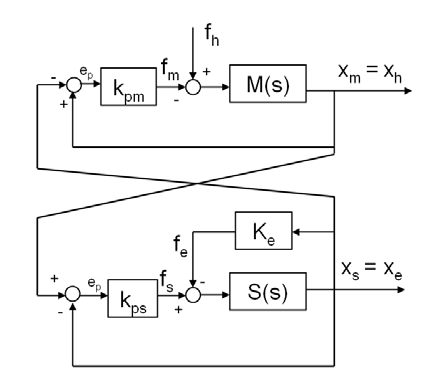
\includegraphics[width=0.6\linewidth]{images/Position-Position.png}
		\caption{Control Posición-Posición.}
		\label{POSPOS}
	\end{figure}
\end{frame}

\begin{frame}{Arquitecturas}{Fuerza-Posición}
	\begin{figure}[h!]
		\centering
		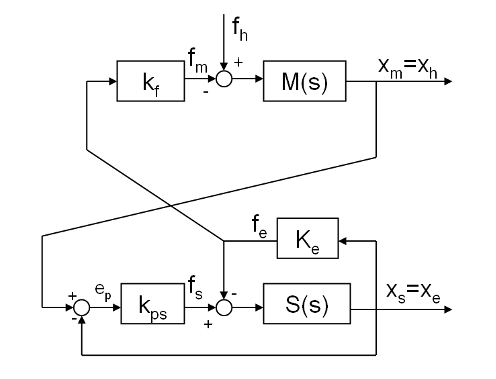
\includegraphics[width=0.6\linewidth]{images/Force-Position.png}
		\caption{Control Fuerza-Posición.}
		\label{FORPOS}
	\end{figure}
\end{frame}

\begin{frame}{Arquitecturas}{Fuerza-Velocidad}
	\begin{figure}[h!]
		\centering
		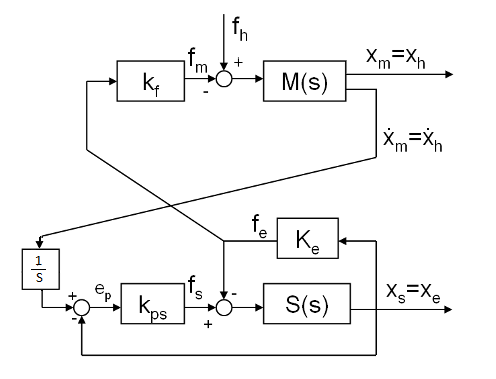
\includegraphics[width=0.6\linewidth]{images/Force-Velocity.png}
		\caption{Control Fuerza-Velocidad}
		\label{FORVEL}
	\end{figure}
\end{frame}

\subsection{Arquitectura de Control con Retraso}

\begin{frame}{El Scattering}{Variables de Onda}
	Retraso en el tiempo de comunicación en un sistema de telerobótica bilateral suele generar inestabilidades.\\
	% Oscilaciones incontroladas especialmente cuando el esclavo está en contacto con objetos en el ambiente remoto.
	\medskip
	La idea básica es transformar el esfuerzo y las variables de flujo mediante transformaciones lineales (Rotación) en \textbf{variables de onda}. Como resultado la comunicación entre dos puertos se convierte en sin pérdidas (pasiva) para una arbitraria constante de tiempo de retraso.\\
	\medskip
	\begin{block}{Fortaleza}
		No tiene que conocerse el valor de la constante de retraso temporal.
	\end{block}
	%La principal fortaleza de este método es que no tiene que conocerse el valor de la constante de retraso temporal.\\
\end{frame}

\begin{frame}{El Scattering}{Variables de Onda}
	Las variables de onda $u$/$v$ están basadas en las variables de \textit{esfuerzo/flujo}, $f$/$v$.
	
	\begin{equation}
		\begin{split}
			u_m&=\dfrac{1}{\sqrt{2b}}(f_m+b \cdot v_m) \qquad u_s=\dfrac{1}{\sqrt{2b}}(f_s+b \cdot v_s)\\
			\omega_m&=\dfrac{1}{\sqrt{2b}}(f_m-b \cdot v_m) \qquad \omega_s=\dfrac{1}{\sqrt{2b}}(f_s-b \cdot v_s)\\
		\end{split}
	\label{Scatter}
	\end{equation}
	
	%
	Donde $b> 0$.
\end{frame}

\begin{frame}{El Scattering}{}
	
	\begin{figure}[h!]
		\centering
		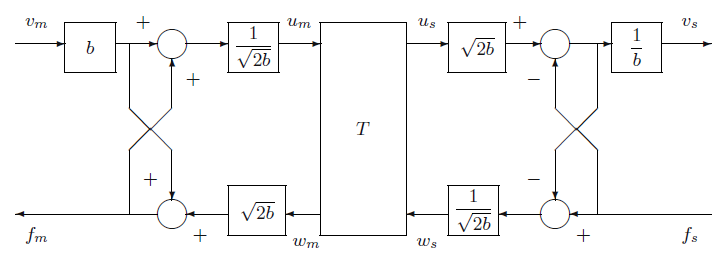
\includegraphics[width=1.0\linewidth]{images/TimeDelay.png}
		\caption{Línea de transmisión basada en la Pasividad}
		\label{DELAY}
	\end{figure}
	
\end{frame}

\begin{frame}{El Scattering}{Adaptación de Impedancias}
	La aplicación de variables de onda en teleoperación implica prestar atención a las \textbf{reflexiones de onda} en ambos lados del telemanipulador, lo cual puede ser evitado por una apropiada \textbf{adaptación de impedancias}.
	
	\begin{equation}
		\begin{split}
		v'_m(t) &= v_m(t)-\dfrac{1}{b}\cdot f_s(t)\\
		f'_s(t) &= f_s(t) + b \cdot v_s(t)
		\end{split}
	\end{equation}
\end{frame}

\begin{frame}{El Scattering}{Adaptación de Impedancias}
	
	\begin{figure}[h!]
		\centering
		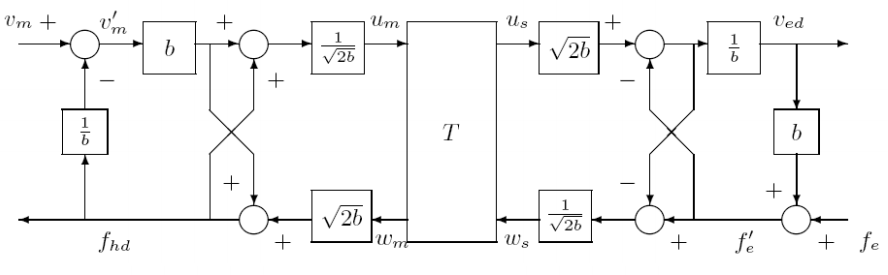
\includegraphics[width=1.0\linewidth]{images/DelayMatch.png}
		\caption{Línea de transmisión basada en la Pasividad con adaptación de impedancias.}
		\label{DELAYMATCH}
	\end{figure}
	
\end{frame}

\section{Simulaciones en Matlab}

\subsection{Modelo}

\begin{frame}{Modelo de Simulink}{Vista General}
	
	\begin{figure}[h!]
		\centering
		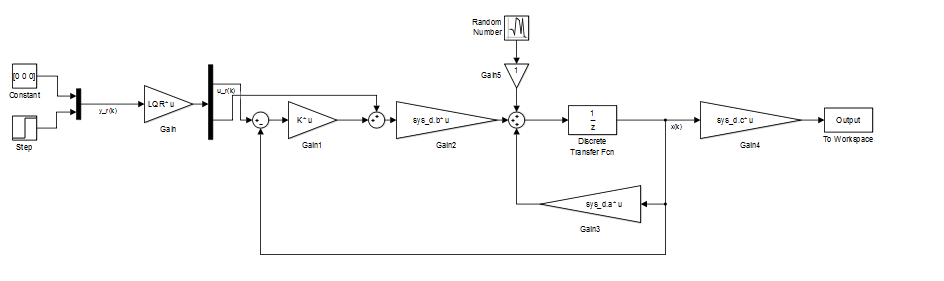
\includegraphics[width=0.7\linewidth]{images/Model.png}
		\caption{Modelo Fuerza-Velocidad con Variables de onda.}
		\label{Model}
	\end{figure}
\end{frame}

\begin{frame}{Modelo de Simulink}{Maestro}
	
	\begin{figure}[h!]
		\centering
		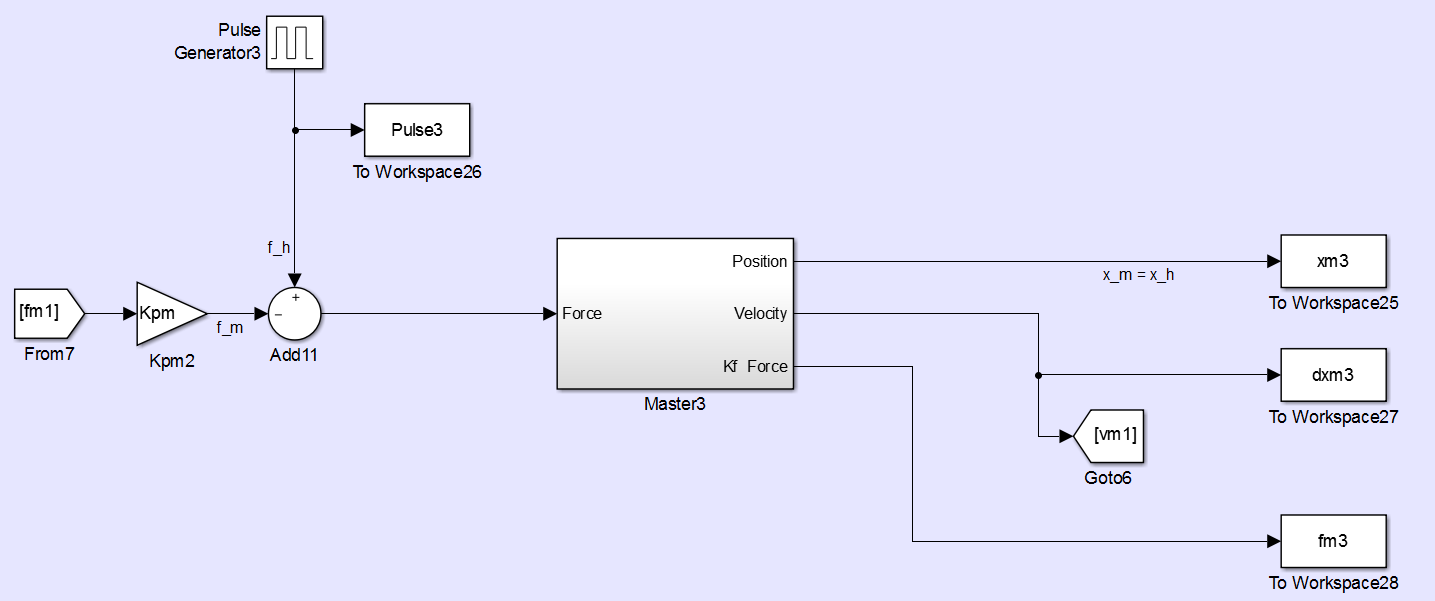
\includegraphics[width=1.0\linewidth]{images/MasterGen.png}
		\caption{Parte del Modelo correspondiente al Maestro.}
		\label{MasterGen}
	\end{figure}
\end{frame}

\begin{frame}{Modelo de Simulink}{Maestro}
	
	\begin{equation}
		M_m \cdot \ddot{x}_m(t) = -K_f \cdot f_{md}(t) - B_m \cdot \dot{x}_m(t) - K_h \cdot x_m(t)
	\end{equation}
	
	\begin{figure}[h!]
		\centering
		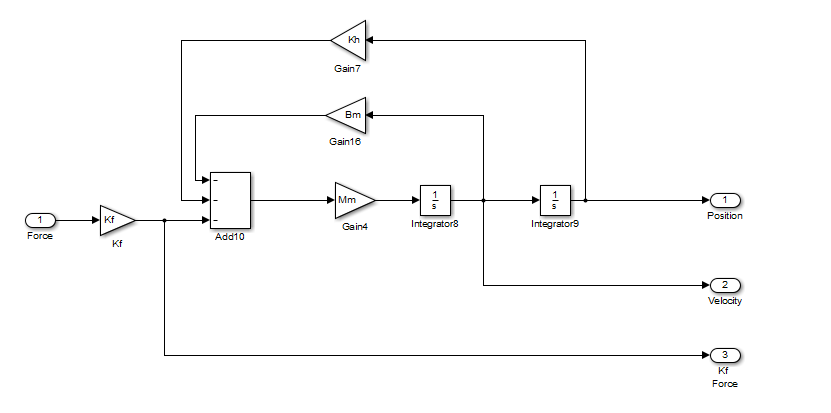
\includegraphics[width=1.0\linewidth]{images/Master.png}
		\caption{Modelo del Maestro.}
		\label{Master}
	\end{figure}
\end{frame}

\begin{frame}{Modelo de Simulink}{Esclavo}
	
	\begin{figure}[h!]
		\centering
		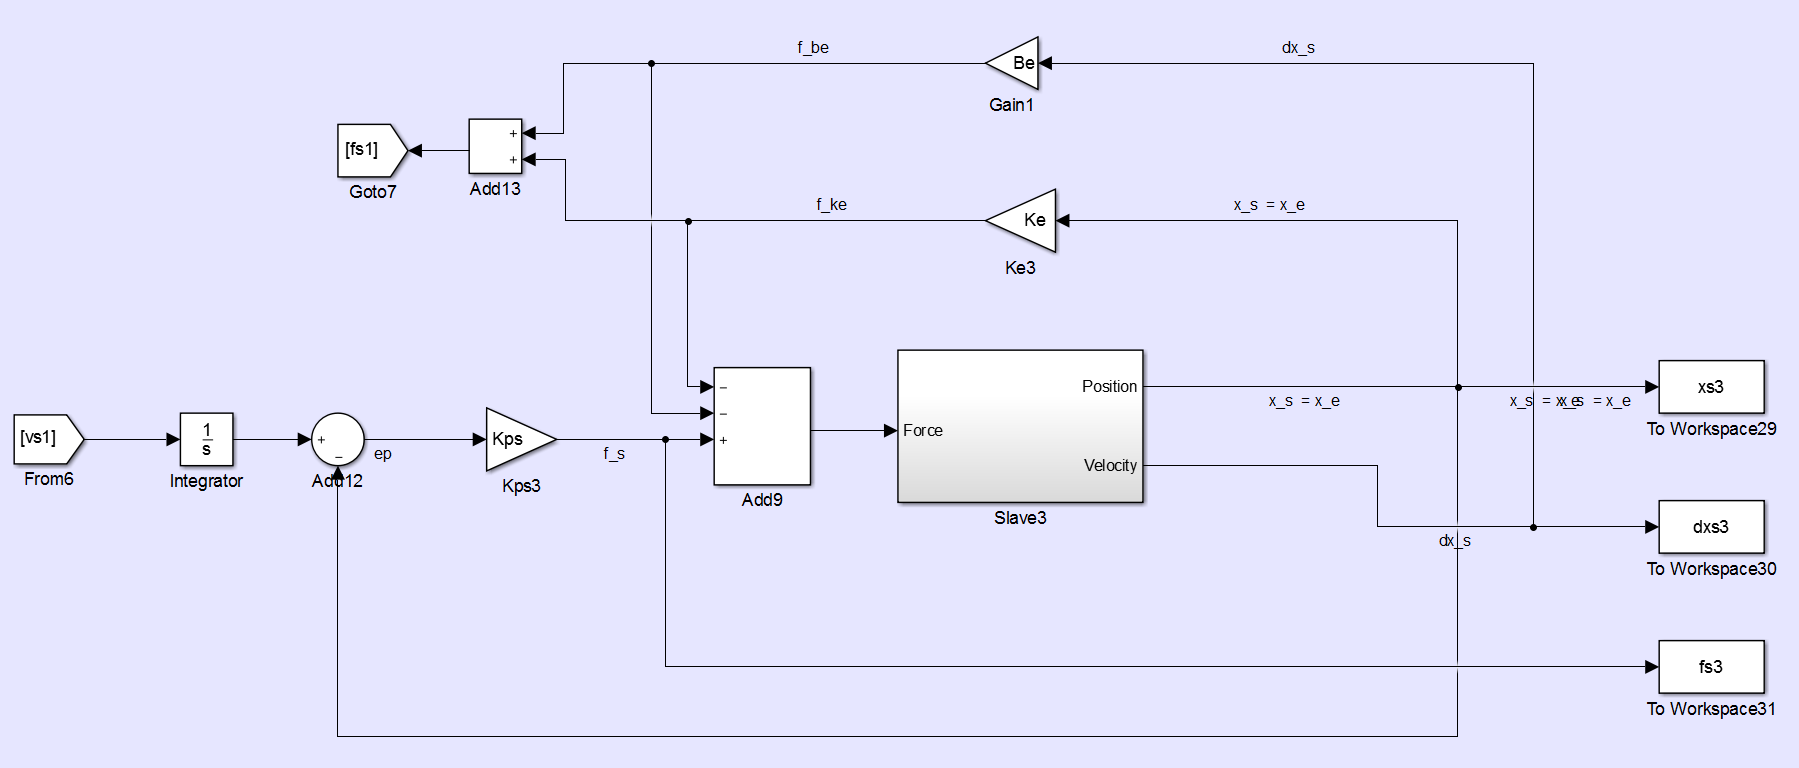
\includegraphics[width=1.0\linewidth]{images/SlaveGen.png}
		\caption{Parte del Modelo correspondiente al Esclavo.}
		\label{SlaveGen}
	\end{figure}
\end{frame}

\begin{frame}{Modelo de Simulink}{Esclavo}
	
	\begin{equation}
	M_s \cdot \ddot{x}_s(t) = f_{s}(t) - B_s \cdot \dot{x}_s(t)
	\end{equation}
	
	\begin{figure}[h!]
		\centering
		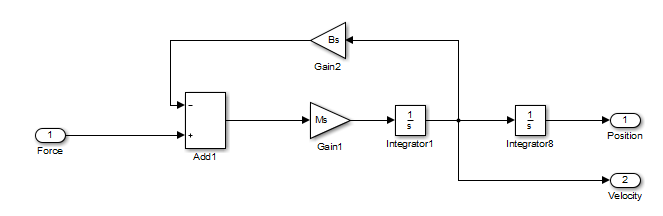
\includegraphics[width=1.0\linewidth]{images/Slave.png}
		\caption{Modelo del Esclavo.}
		\label{Slave}
	\end{figure}
\end{frame}

\begin{frame}{Modelo de Simulink}{Modelo de Línea de Transmisión}
	
	\begin{figure}[h!]
		\centering
		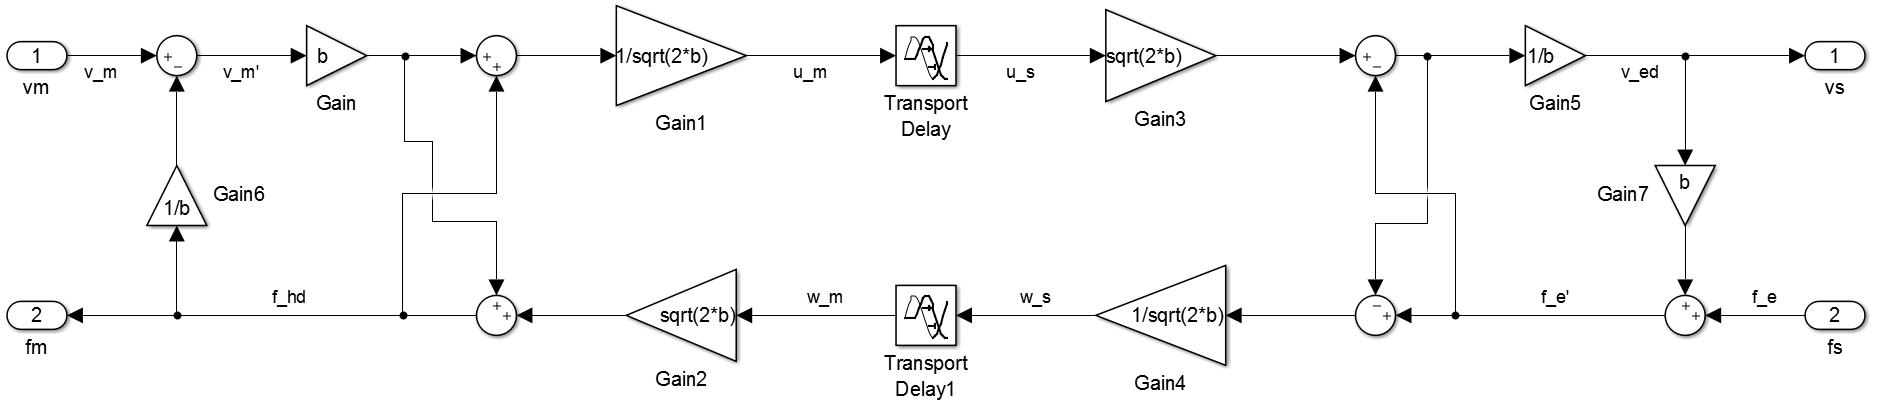
\includegraphics[width=1.0\linewidth]{images/Transmission.png}
		\caption{Línea de Transmisión basada en Pasividad [\ref{Scatter}].}
		\label{Transmision}
	\end{figure}
\end{frame}

\begin{frame}{Variables Usadas}
	
	\begin{equation}
		\begin{split}
		B_m = B_s = 20 \qquad &Coeficientes\ de\ Fricci\acute{o}n\\
		K_h = 0 \qquad &Constante\ El\acute{a}stica\ del\ Master\\
		K_{pm} = 0.1;\ K_{ps} = 100 \qquad &Constantes\ Proporcionales\\
		M_m = M_s = 1 \qquad &Masas\\
		K_e = B_e = 0.25 \qquad &Constantes\ del \ Entorno\\
		K_f = 100; 	\qquad &Otra\ Constante\ Porporcional\ del\ Master\\
		T_d = 1.0 \qquad &Tiempo\ de\ Retraso\\
		b = 0.2 \qquad &Constante\ b\ de\ Scattering
		\end{split}
	\end{equation}
	
\end{frame}

\subsection{Simulaciones y Resultados}

\begin{frame}{Variando el Tiempo de Retraso}{$T_d=2$}
	
	\begin{figure}[h!]
		\centering
		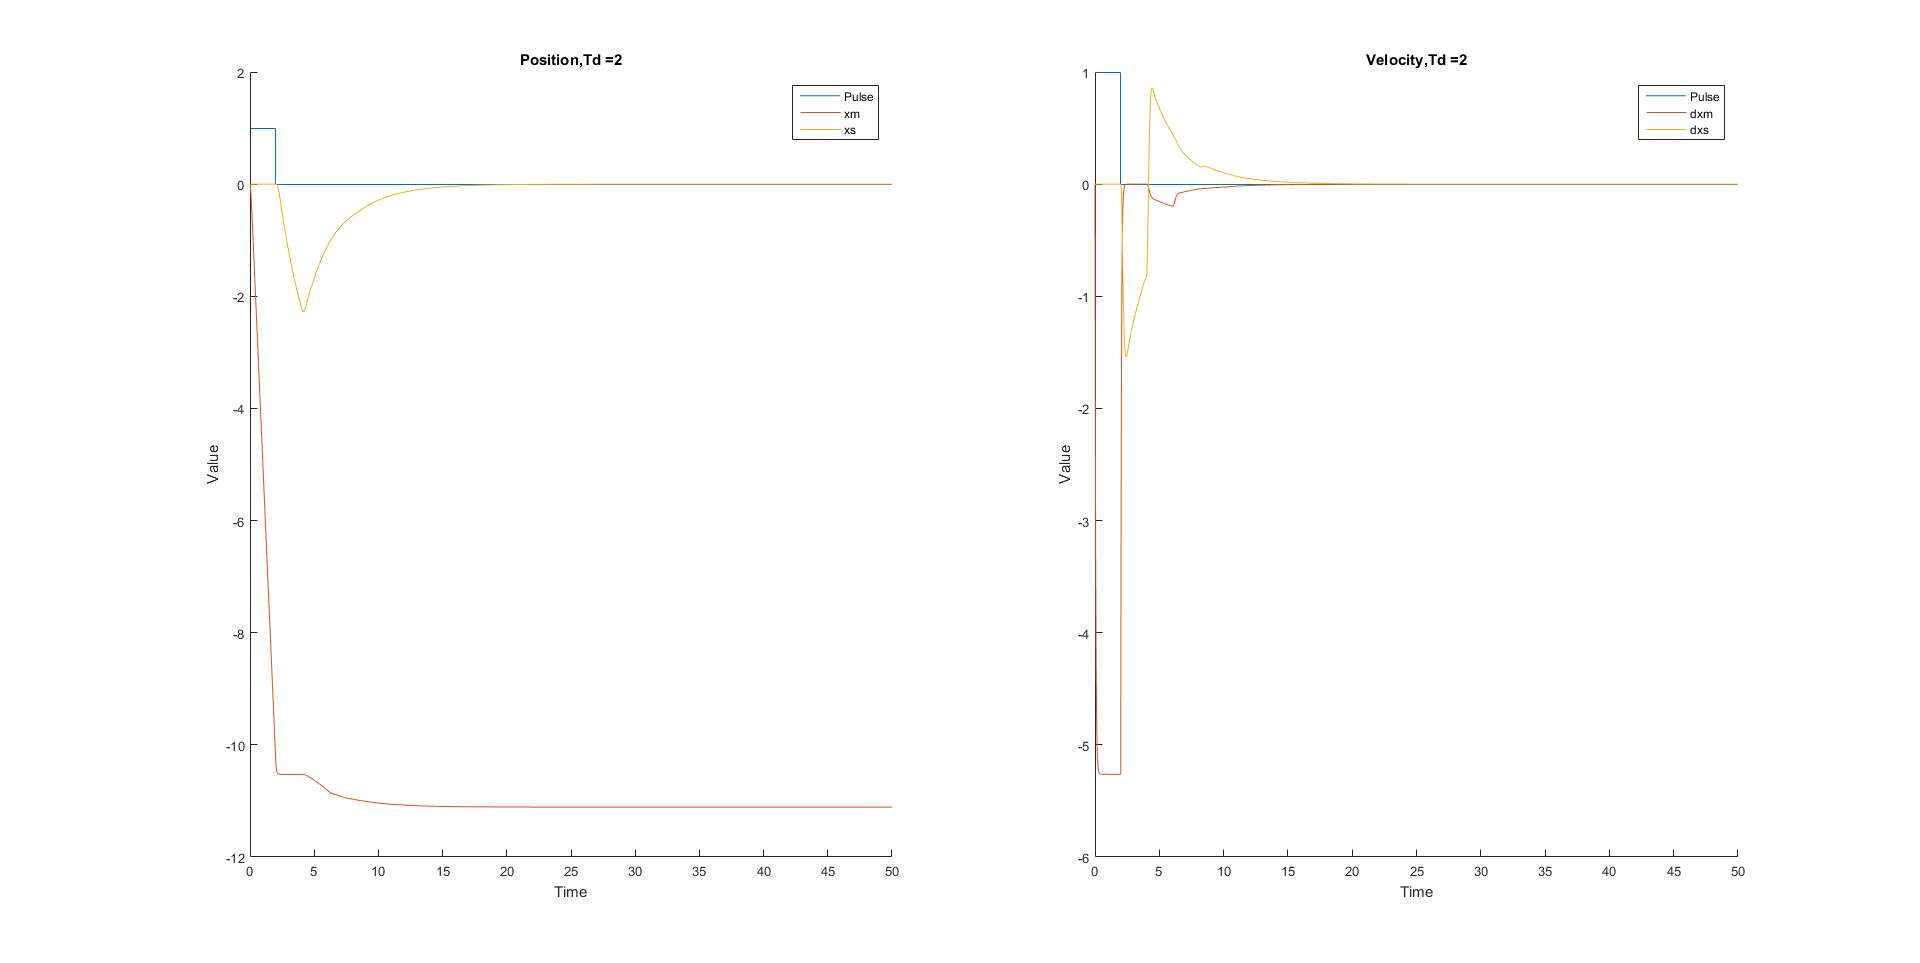
\includegraphics[width=1.0\linewidth]{images/Td2.png}
		\caption{Tiempo de Retraso, $T_d=2$}
		\label{TD2}
	\end{figure}
	
\end{frame}

\begin{frame}{Variando el Tiempo de Retraso}{$T_d=10$}
	
	\begin{figure}[h!]
		\centering
		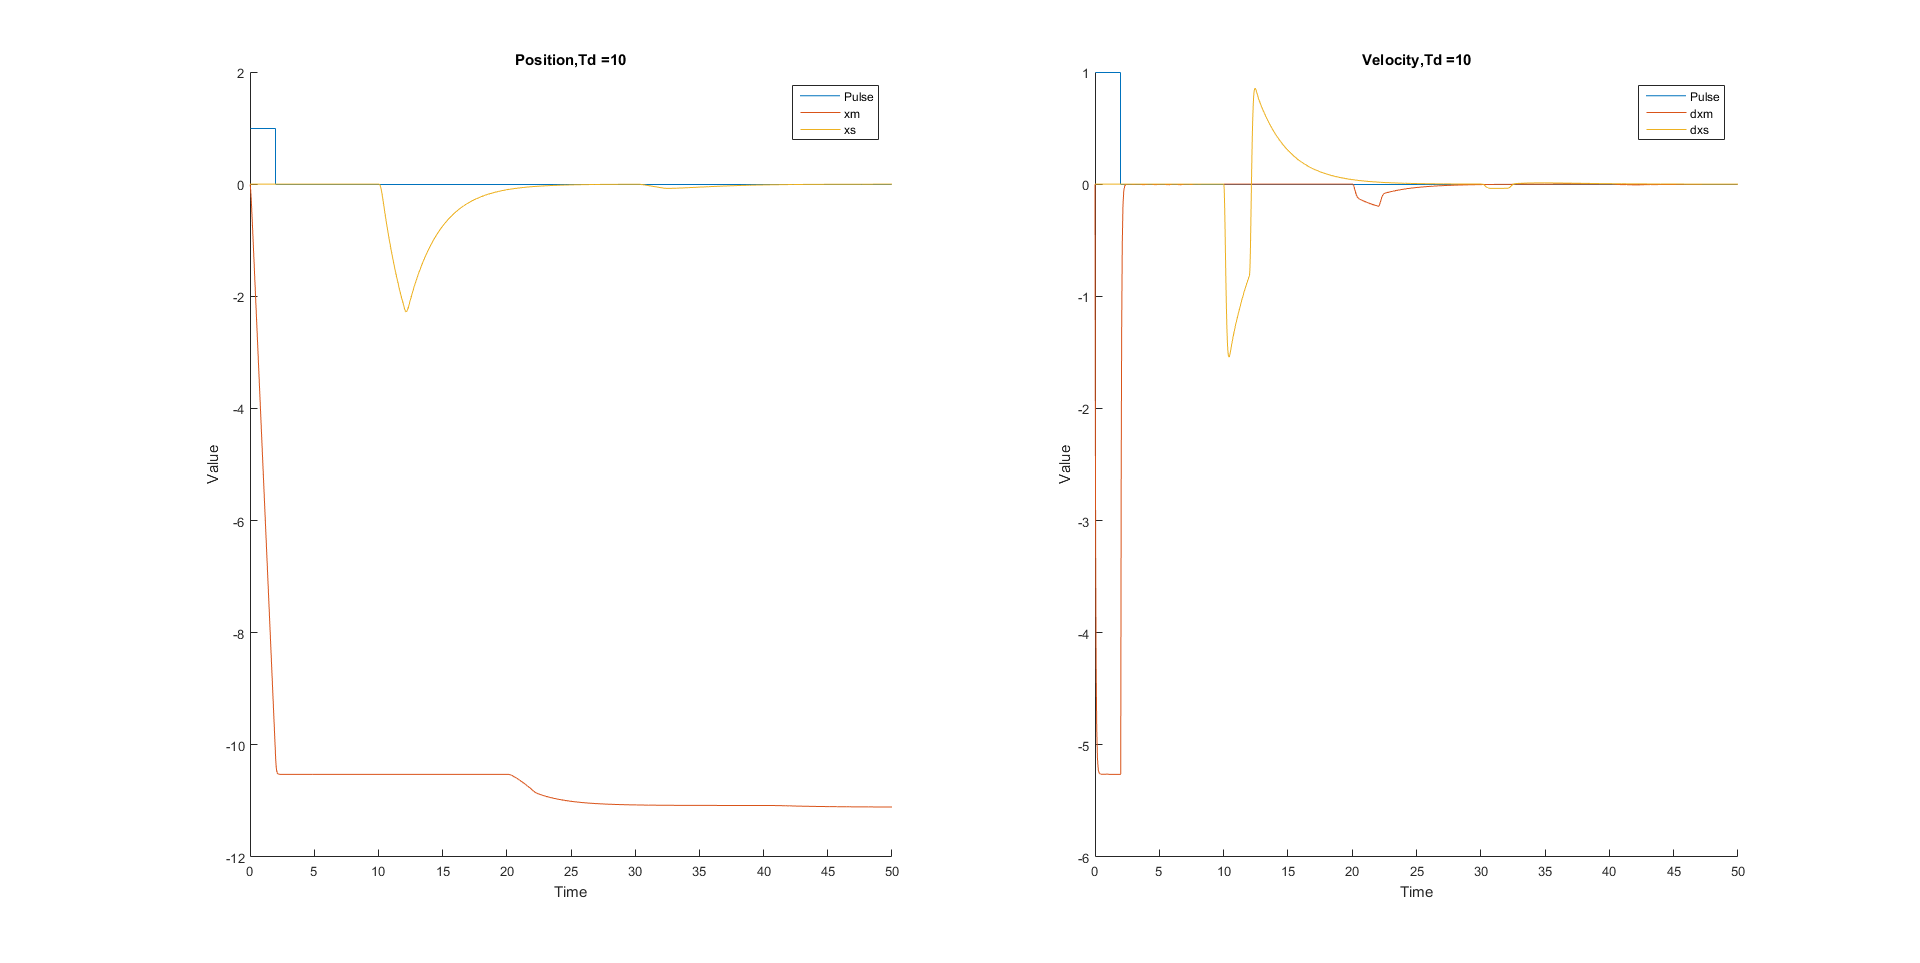
\includegraphics[width=1.0\linewidth]{images/Td10.png}
		\caption{Tiempo de Retraso, $T_d=10$}
		\label{TD10}
	\end{figure}
	
\end{frame}

\begin{frame}{Variando el Tiempo de Retraso}{$T_d=20$}
	
	\begin{figure}[h!]
		\centering
		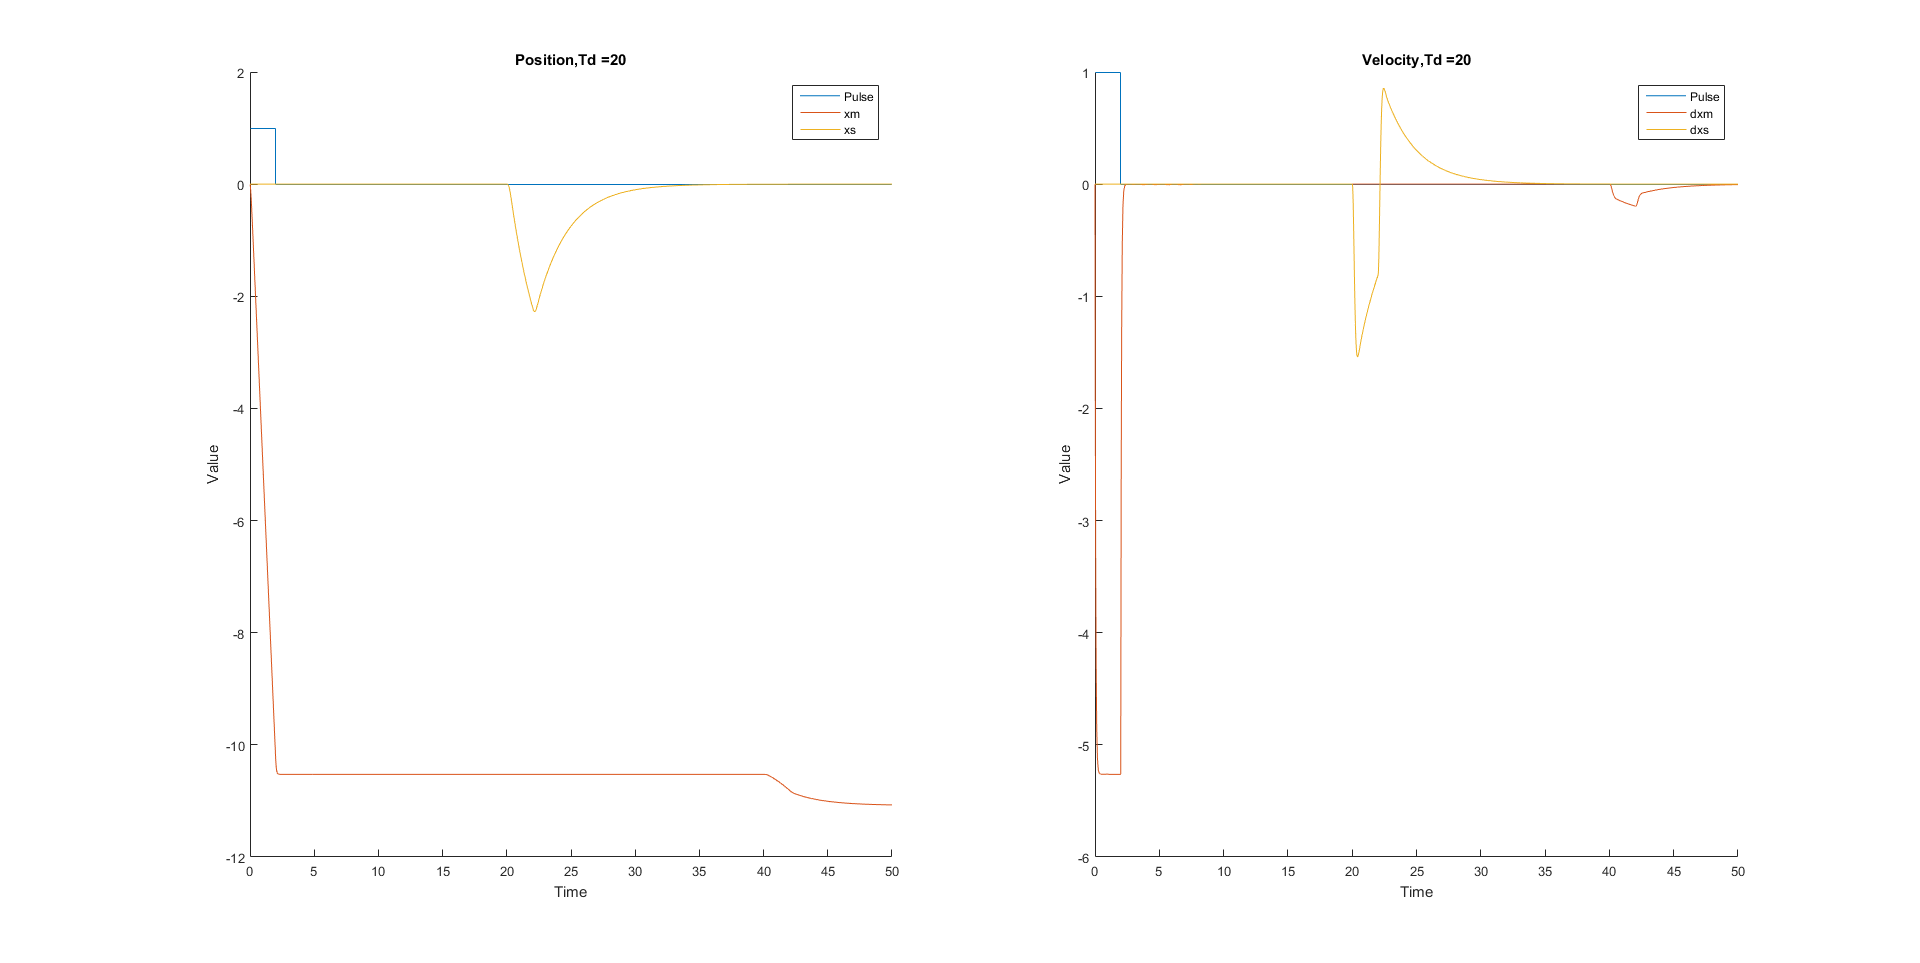
\includegraphics[width=1.0\linewidth]{images/Td20.png}
		\caption{Tiempo de Retraso, $T_d=20$}
		\label{TD20}
	\end{figure}
	
\end{frame}

\begin{frame}{Variando la constante $b$ de Scattering}{$b=0.2$}
	
	\begin{figure}[h!]
		\centering
		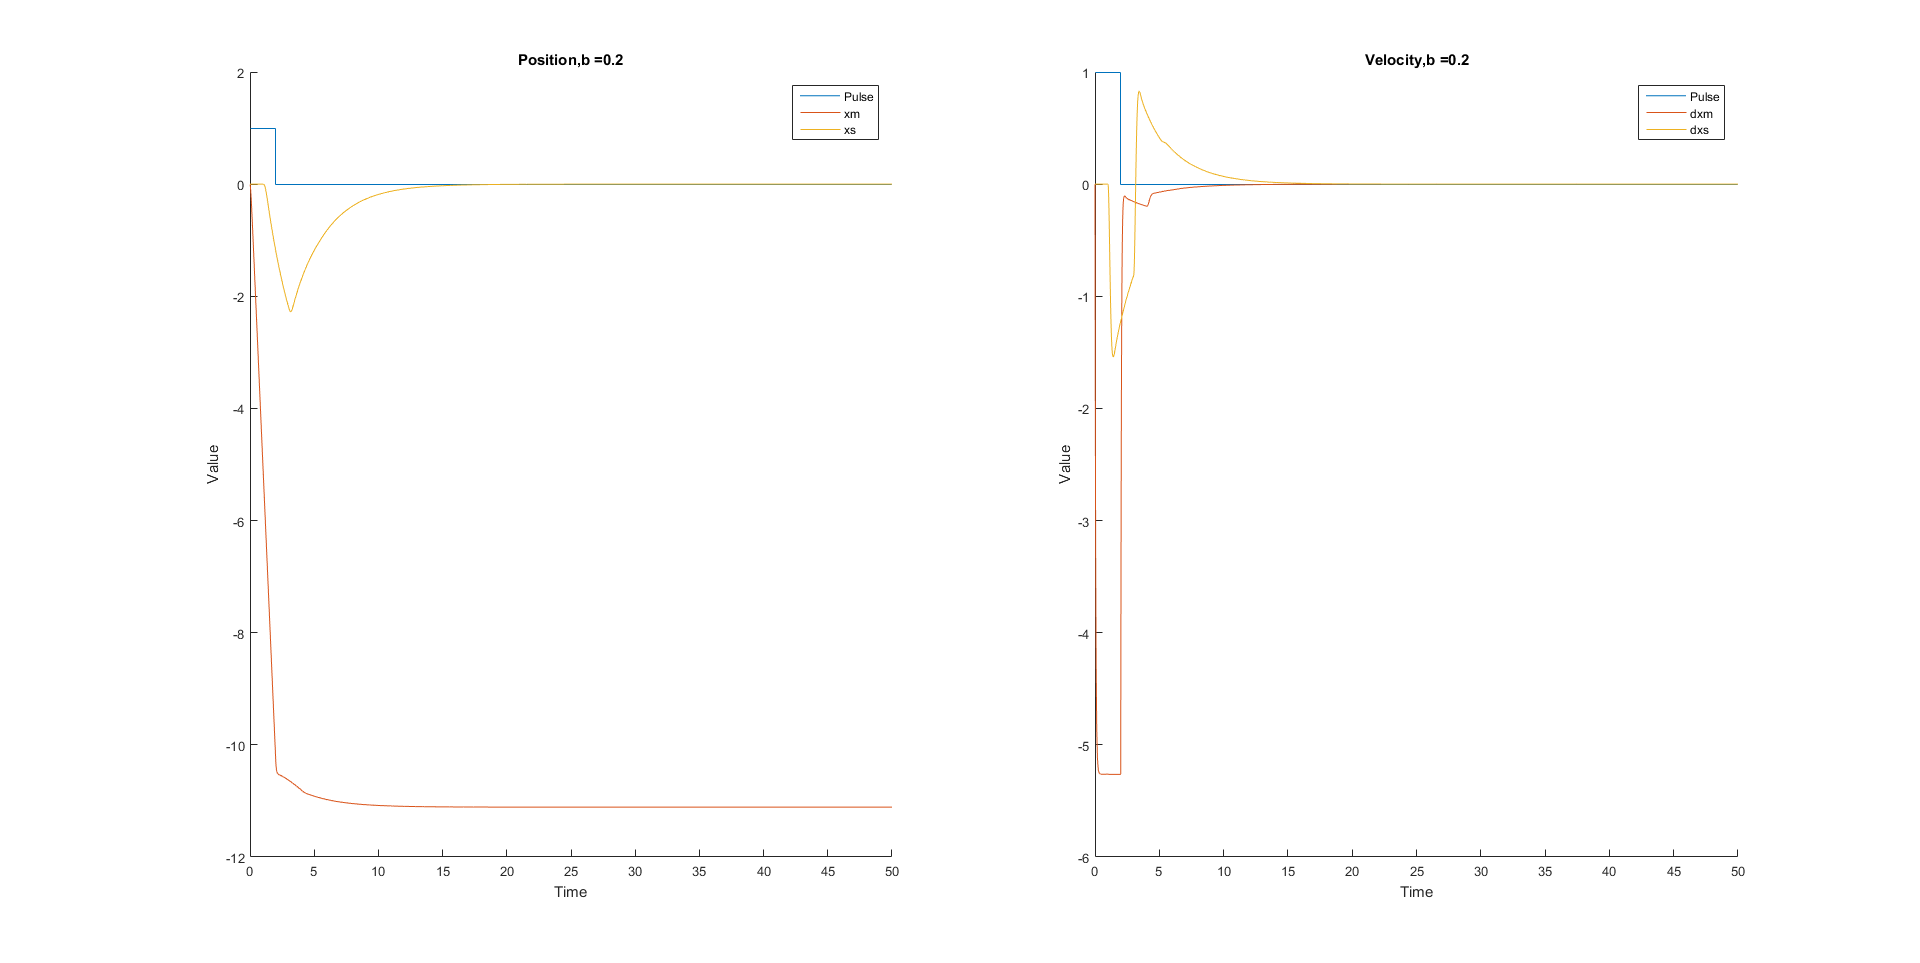
\includegraphics[width=1.0\linewidth]{images/b02.png}
		\caption{Constante $b$ de Scattering, $b=0.2$}
		\label{B02}
	\end{figure}
	
\end{frame}

\begin{frame}{Variando la constante $b$ de Scattering}{$b=1$}
	
	\begin{figure}[h!]
		\centering
		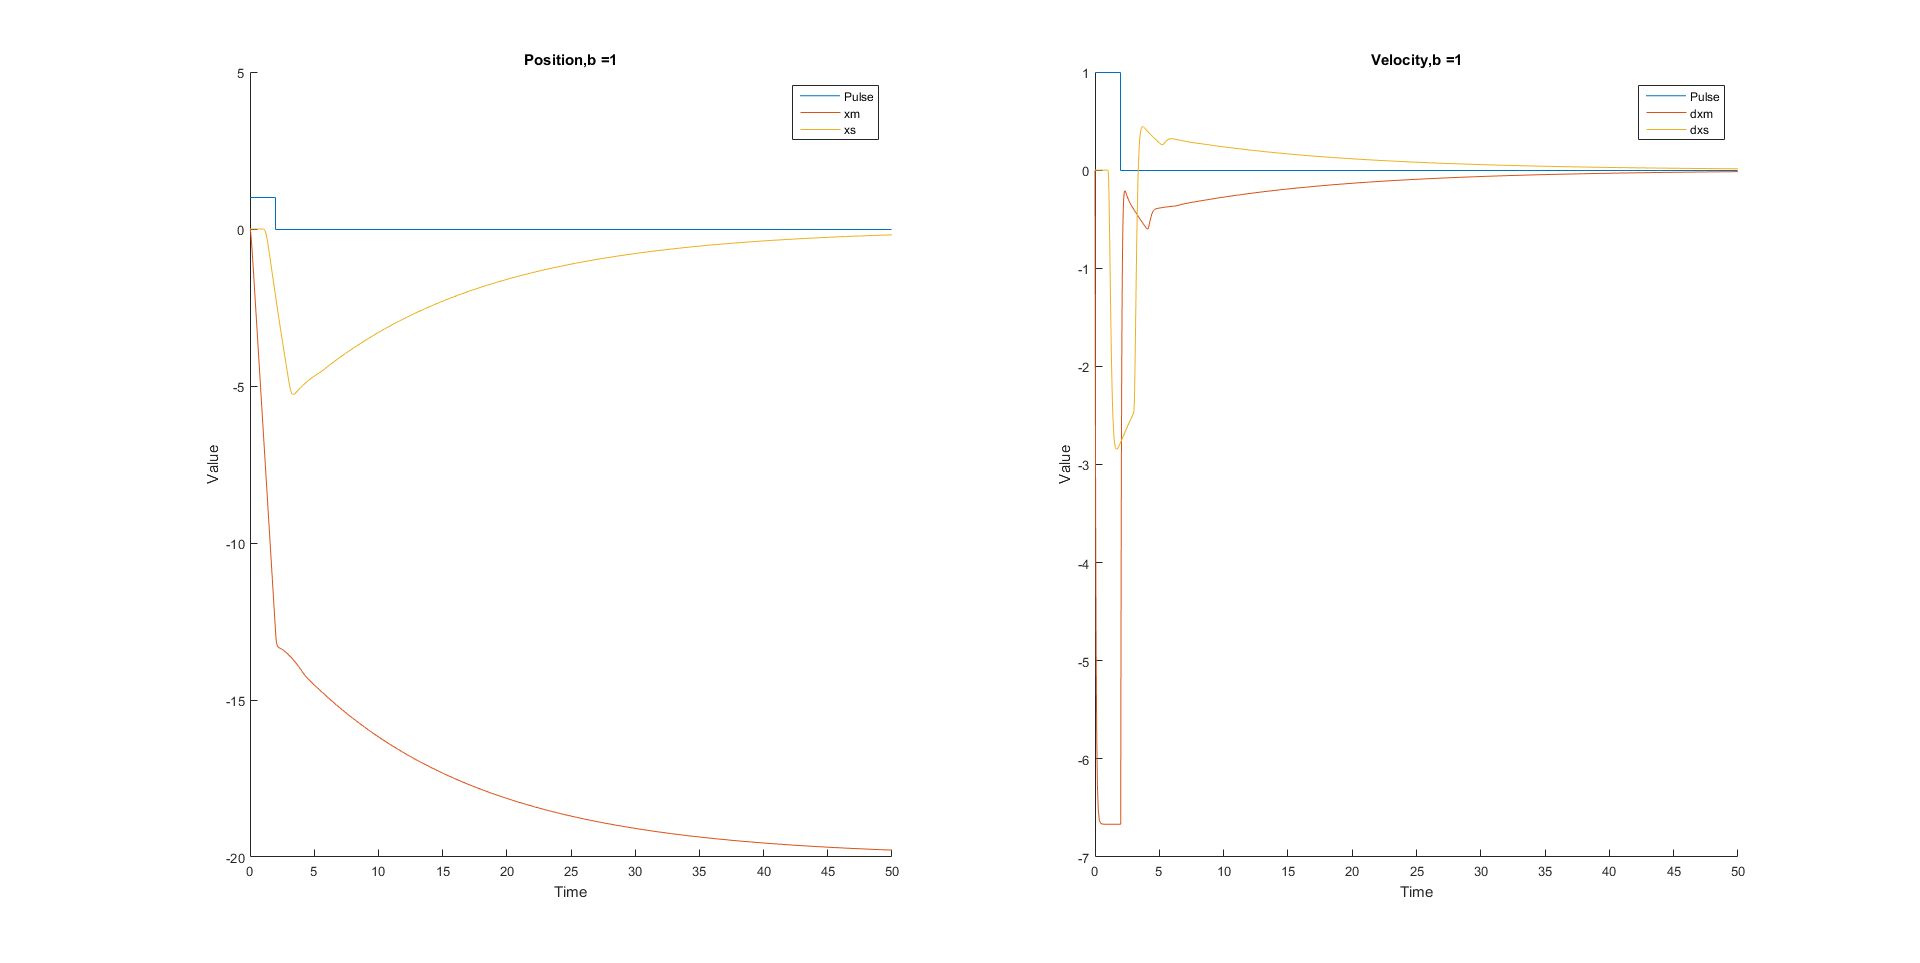
\includegraphics[width=1.0\linewidth]{images/b1.png}
		\caption{Constante $b$ de Scattering, $b=1$}
		\label{B1}
	\end{figure}
	
\end{frame}

\begin{frame}{Variando la constante $b$ de Scattering}{$b=2$}
	
	\begin{figure}[h!]
		\centering
		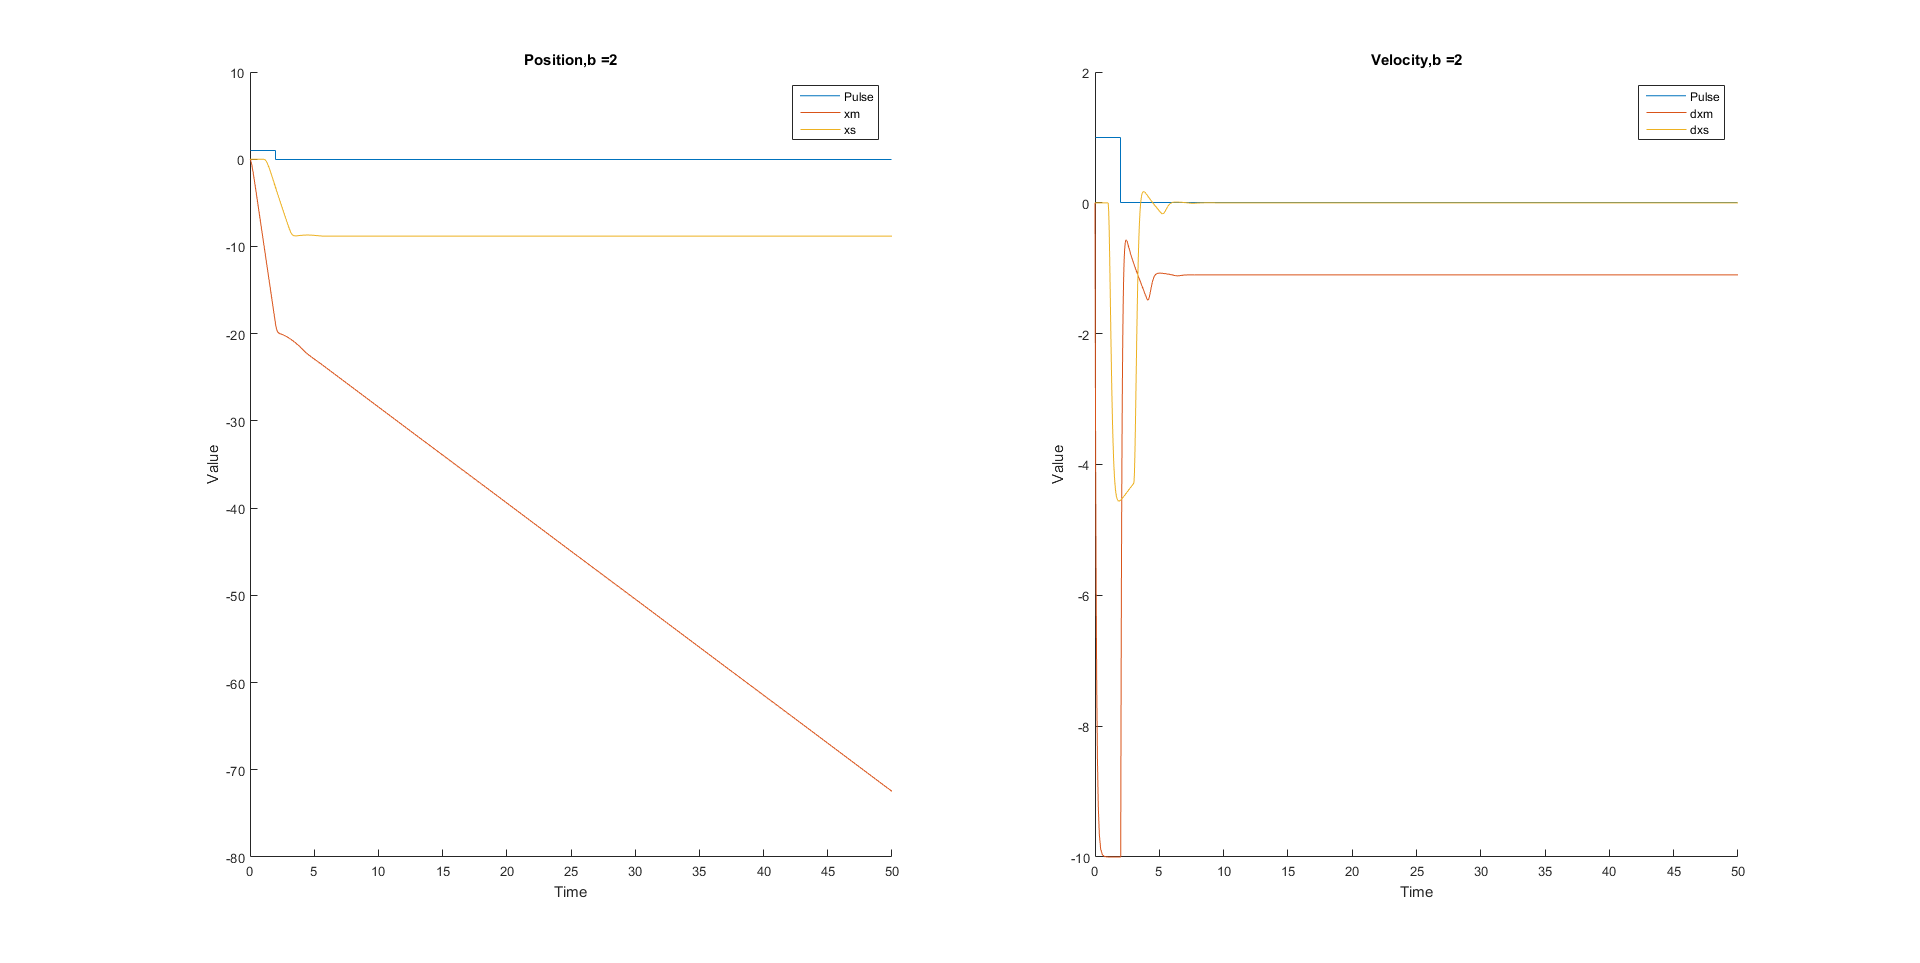
\includegraphics[width=1.0\linewidth]{images/b2.png}
		\caption{Constante $b$ de Scattering, $b=2$}
		\label{B2}
	\end{figure}
	
\end{frame}

\begin{frame}{Variando la Masa del Esclavo}{$M_s=1$}
	
	\begin{figure}[h!]
		\centering
		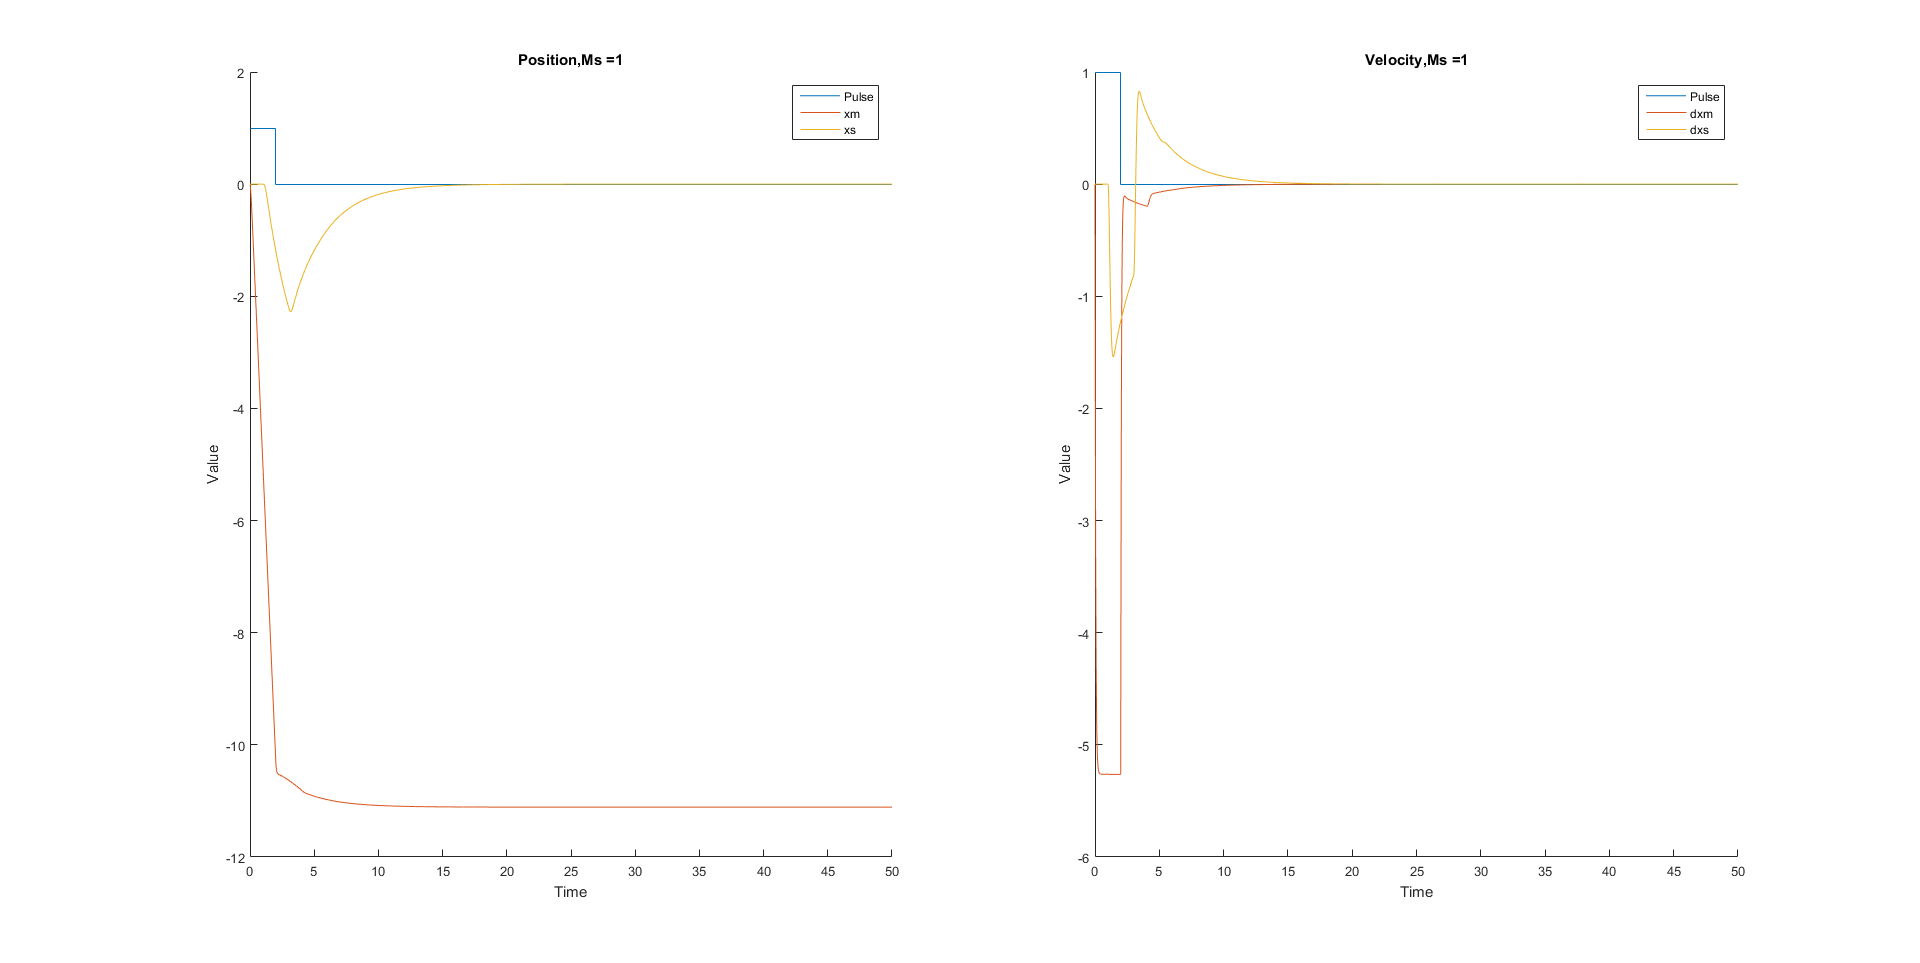
\includegraphics[width=1.0\linewidth]{images/Ms1.png}
		\caption{Masa del Esclavo, $M_s=1$}
		\label{MS1}
	\end{figure}
	
\end{frame}

\begin{frame}{Variando la Masa del Esclavo}{$M_s=10$}

\begin{figure}[h!]
	\centering
	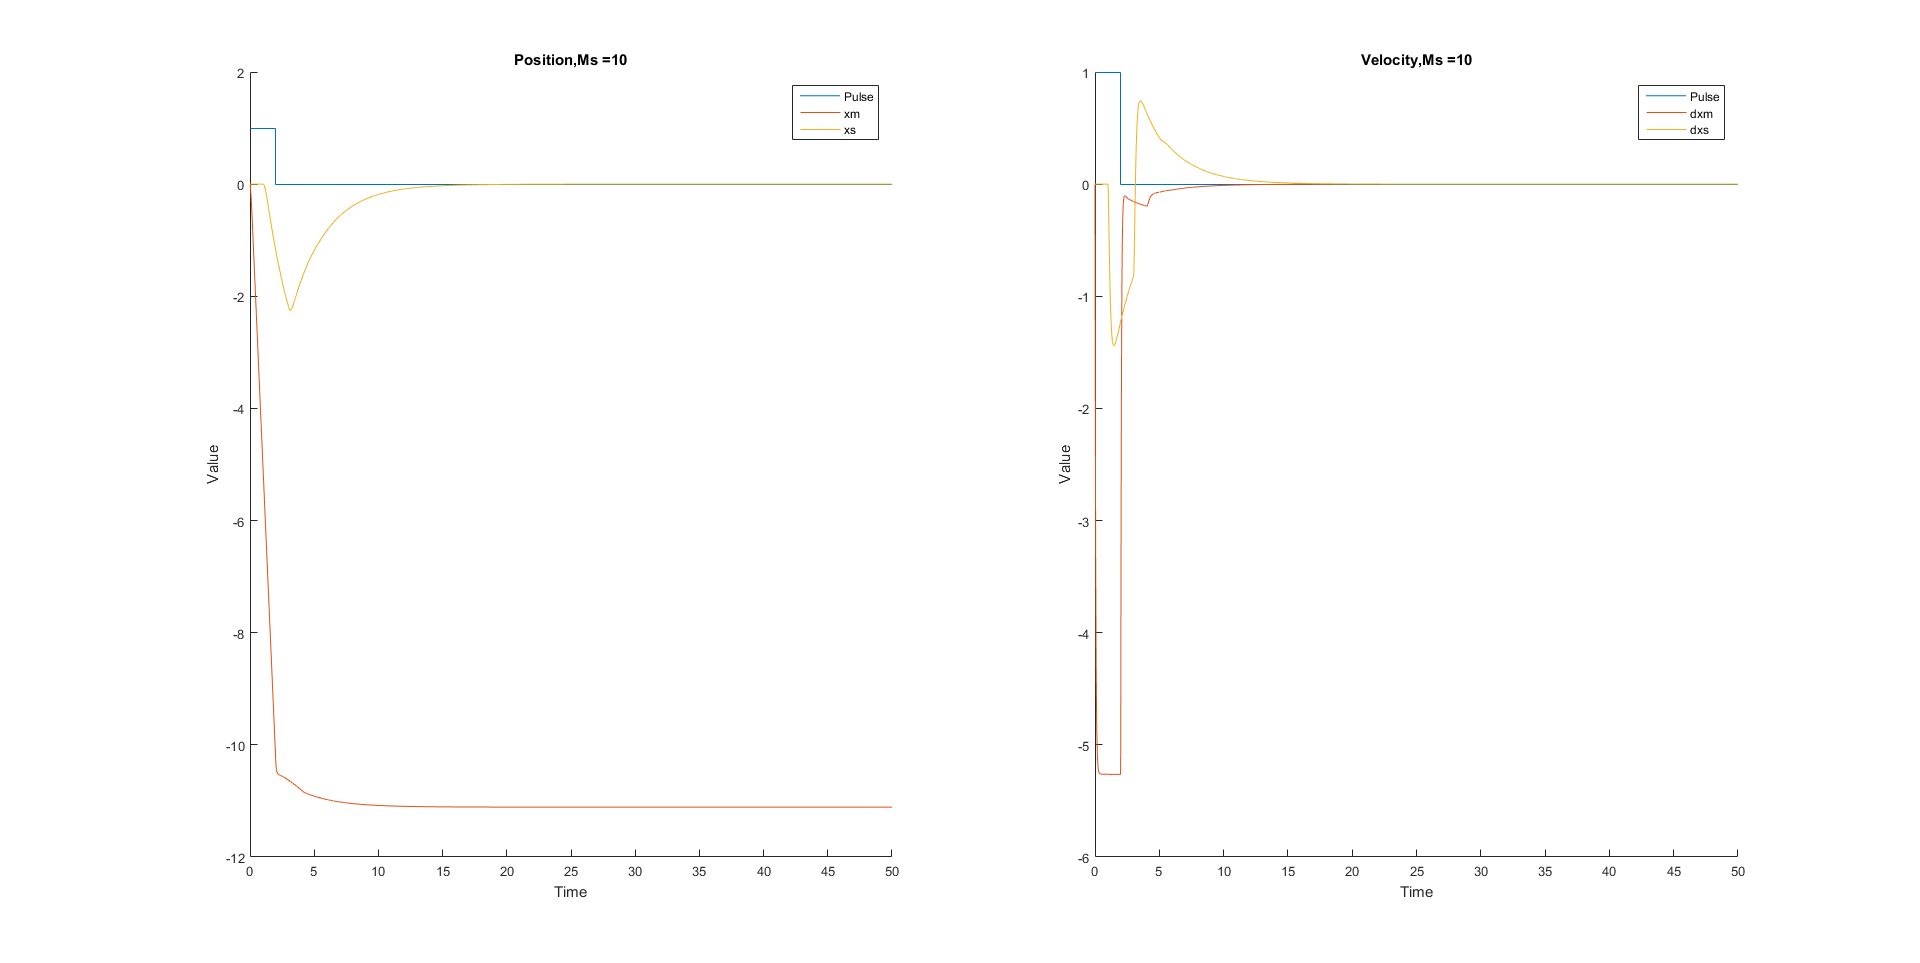
\includegraphics[width=1.0\linewidth]{images/Ms10.png}
	\caption{Masa del Esclavo, $M_s=10$}
	\label{MS10}
\end{figure}

\end{frame}

\begin{frame}{Variando la Constante Elástica del Entorno}{$K_e=0.25$}
	
	\begin{figure}[h!]
		\centering
		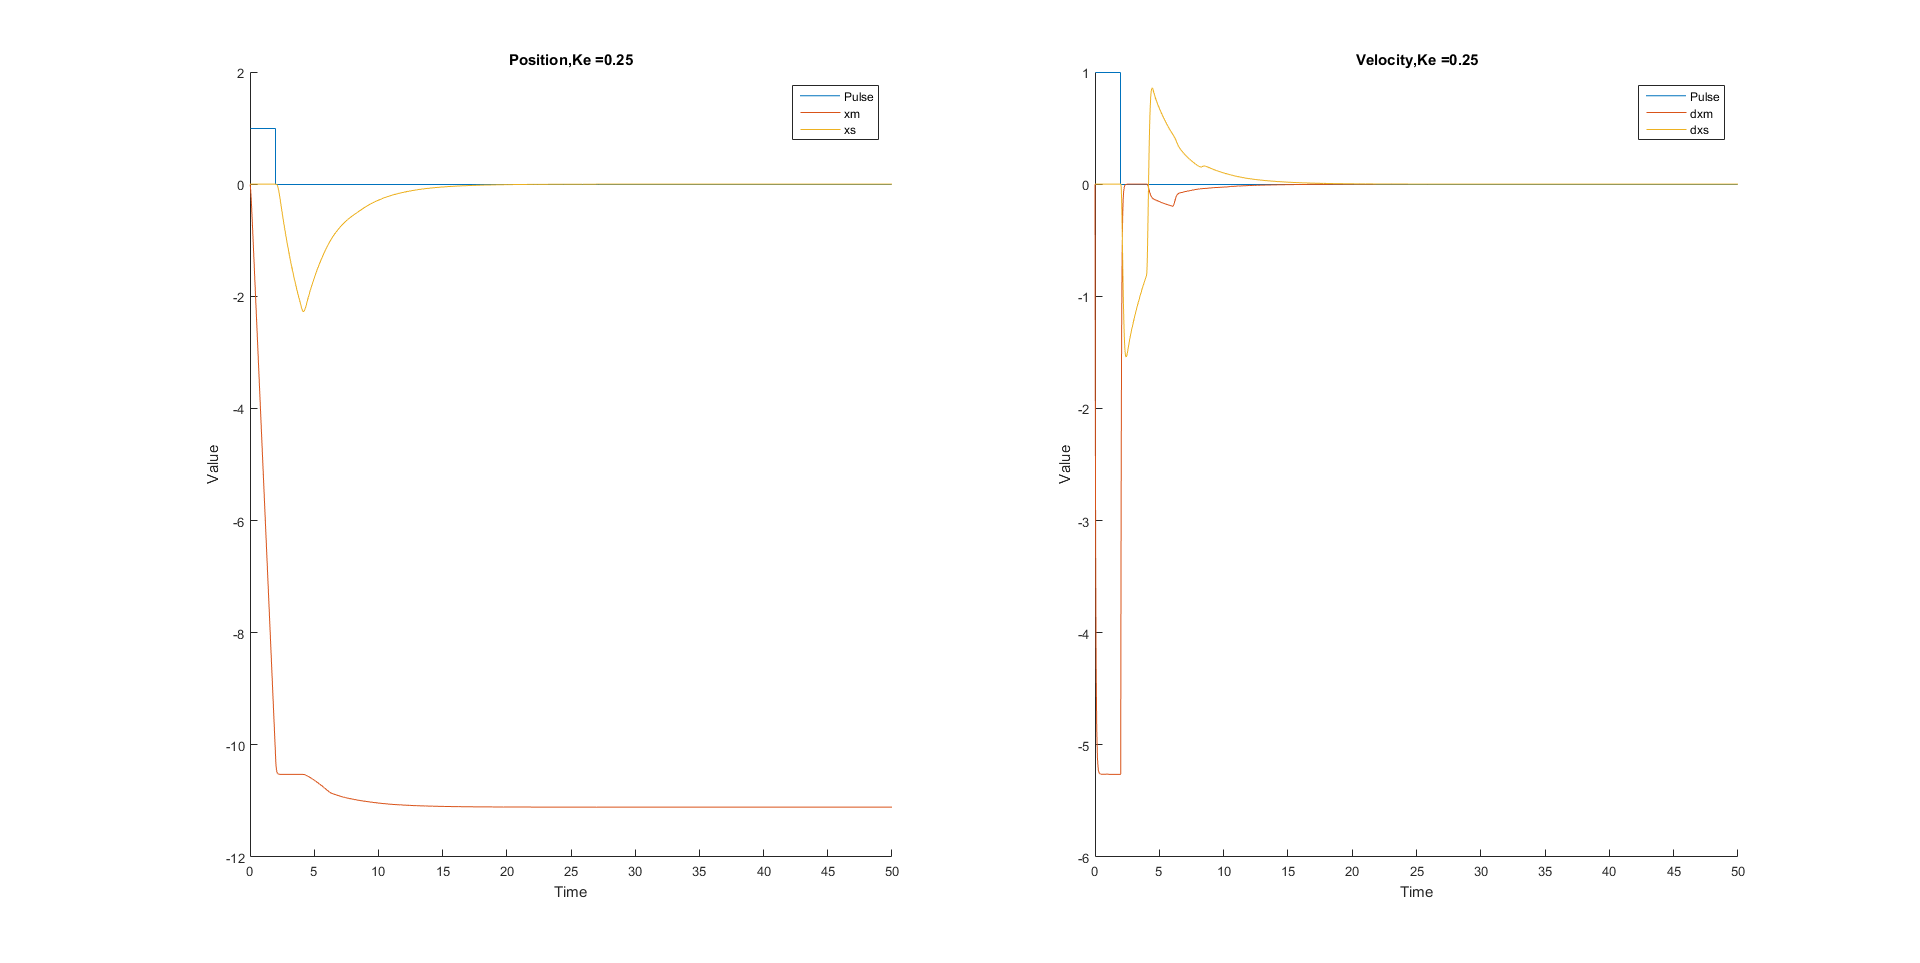
\includegraphics[width=1.0\linewidth]{images/Ke025.png}
		\caption{Constante Elástica del Entorno, $K_e=0.25$}
		\label{KE025}
	\end{figure}
	
\end{frame}

\begin{frame}{Variando la Constante Elástica del Entorno}{$K_e=2.5$}
	
	\begin{figure}[h!]
		\centering
		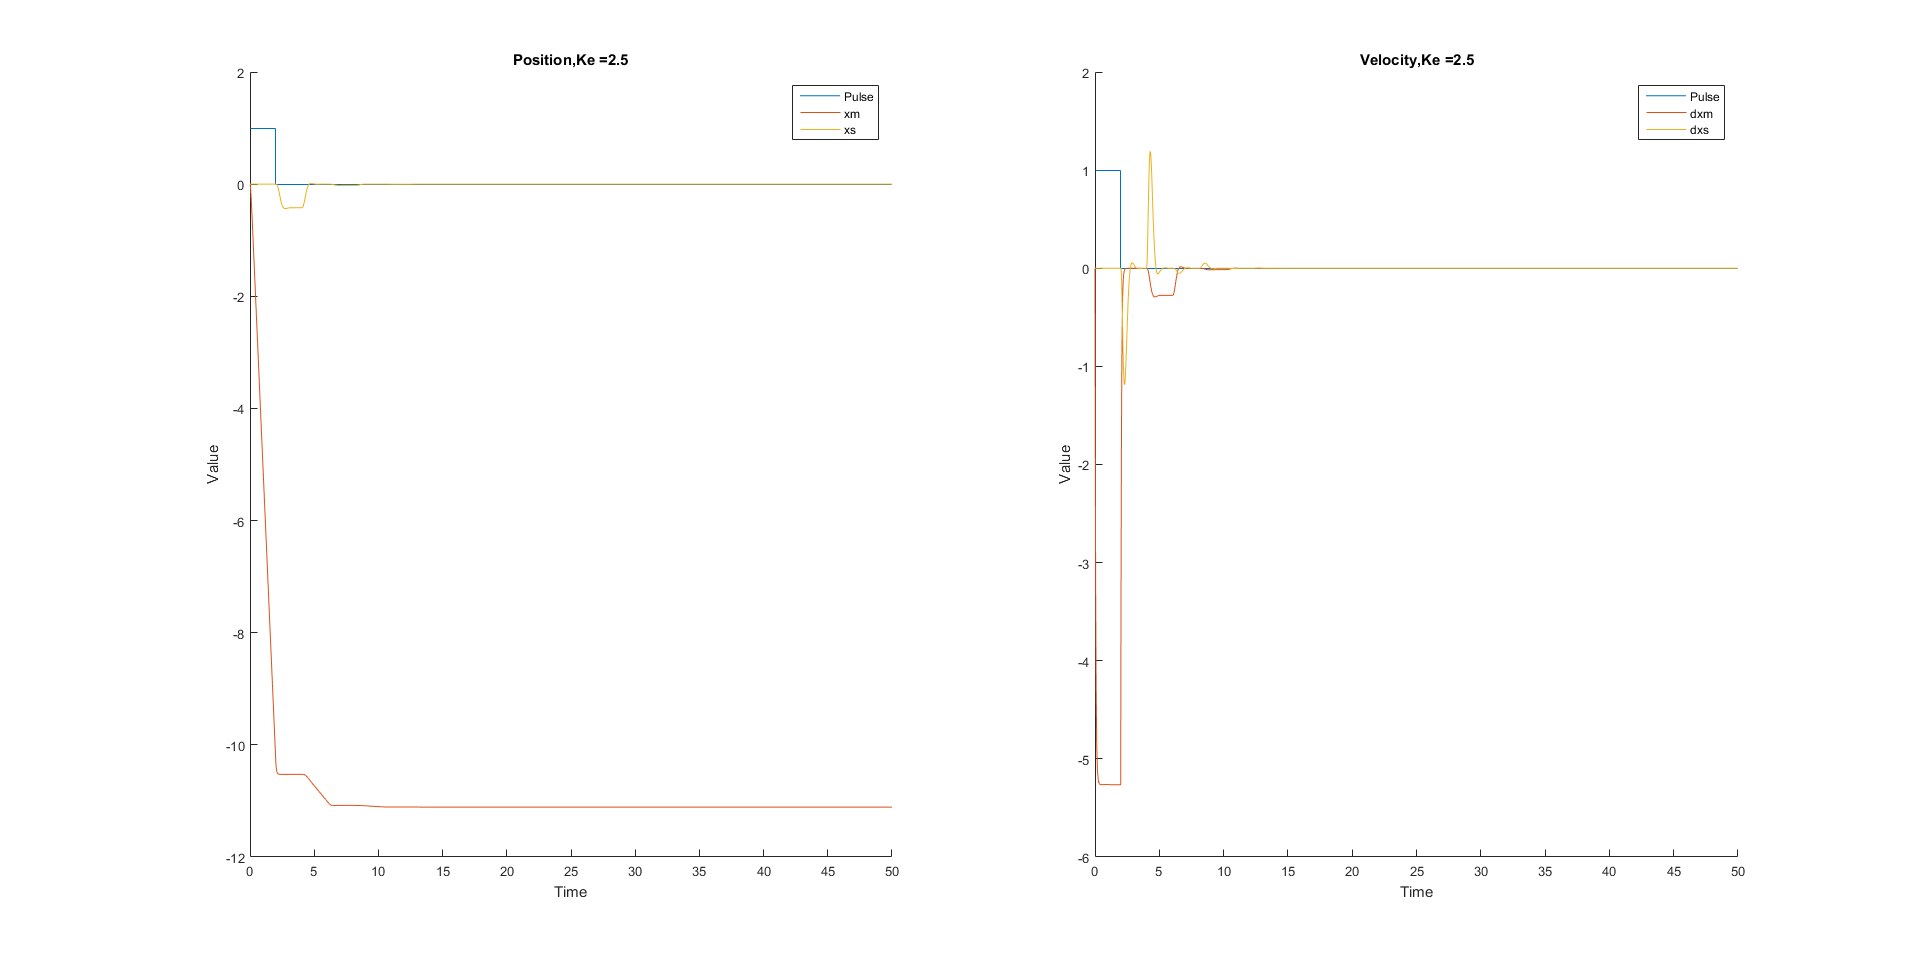
\includegraphics[width=1.0\linewidth]{images/Ke25.png}
		\caption{Constante Elástica del Entorno, $K_e=2.5$}
		\label{KE25}
	\end{figure}
	
\end{frame}

\begin{frame}{Variando la Constante Elástica del Entorno}{$K_e=0$}
	
	\begin{figure}[h!]
		\centering
		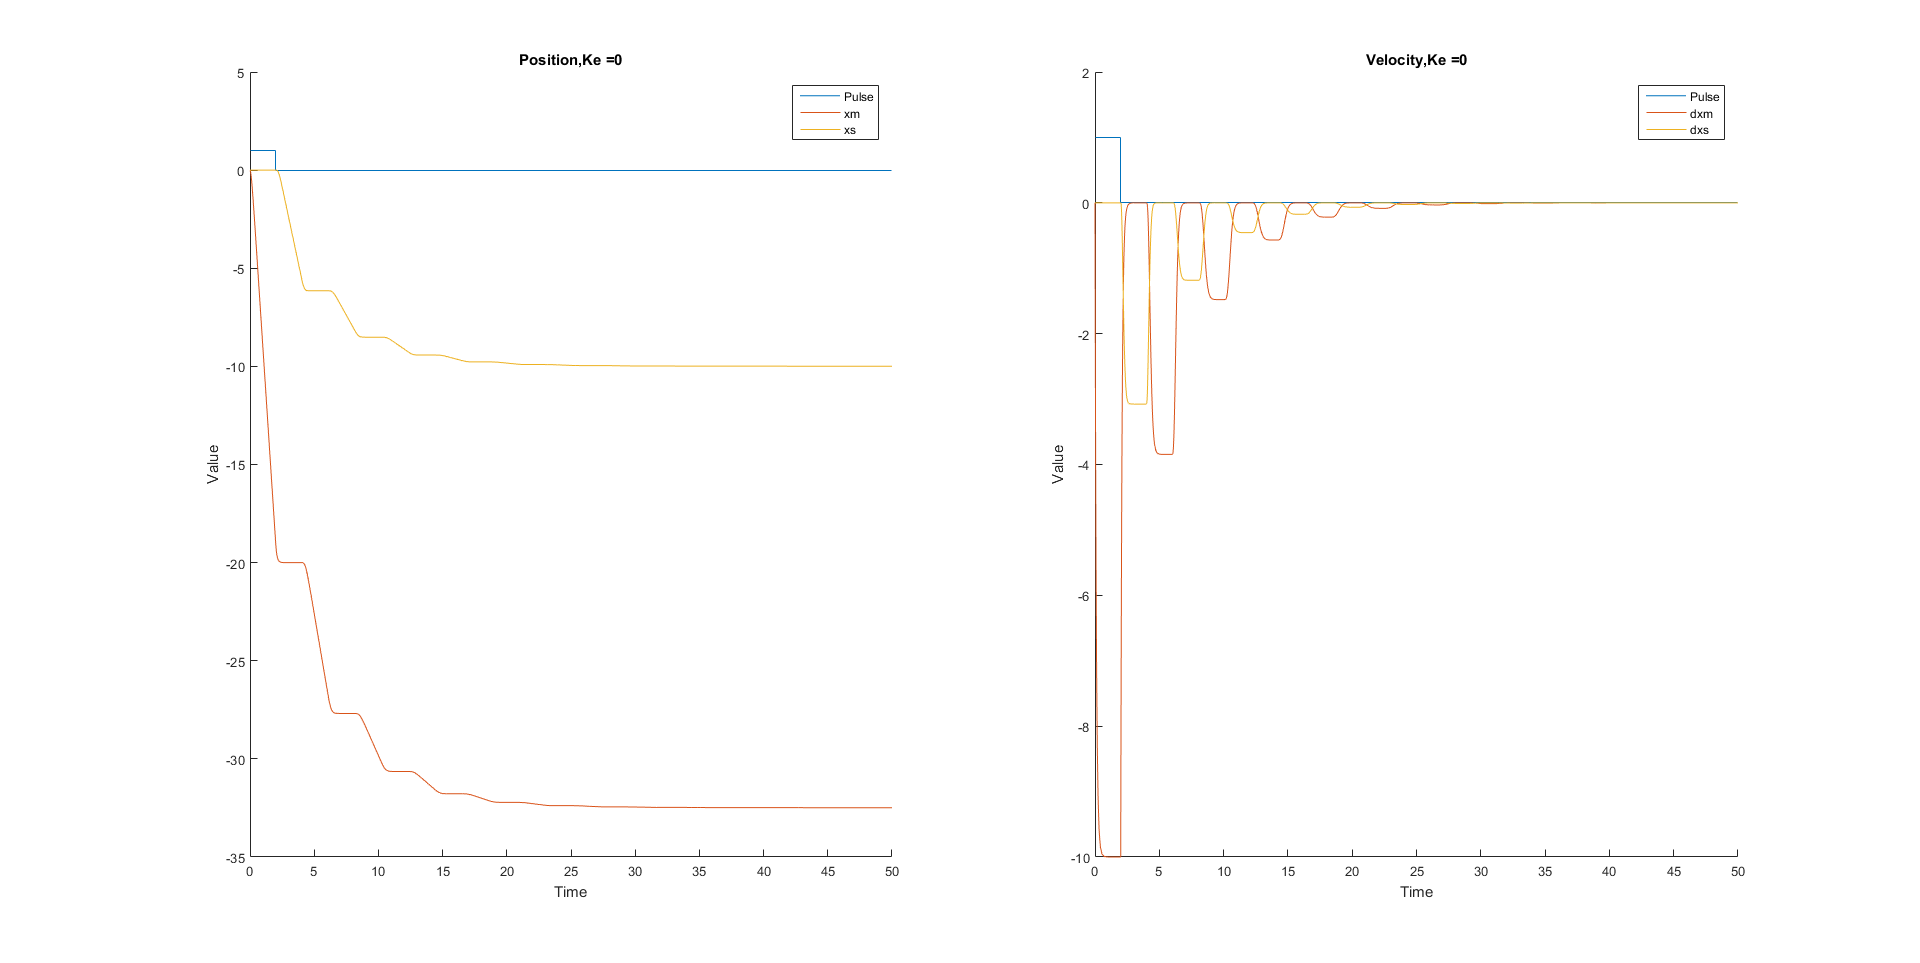
\includegraphics[width=1.0\linewidth]{images/Ke0.png}
		\caption{Constante Elástica del Entorno, $K_e=0$}
		\label{KE0}
	\end{figure}
	
\end{frame}

\begin{frame}{Variando la Constante Fricción del Entorno}{$B_e=0.25$}
	
	\begin{figure}[h!]
		\centering
		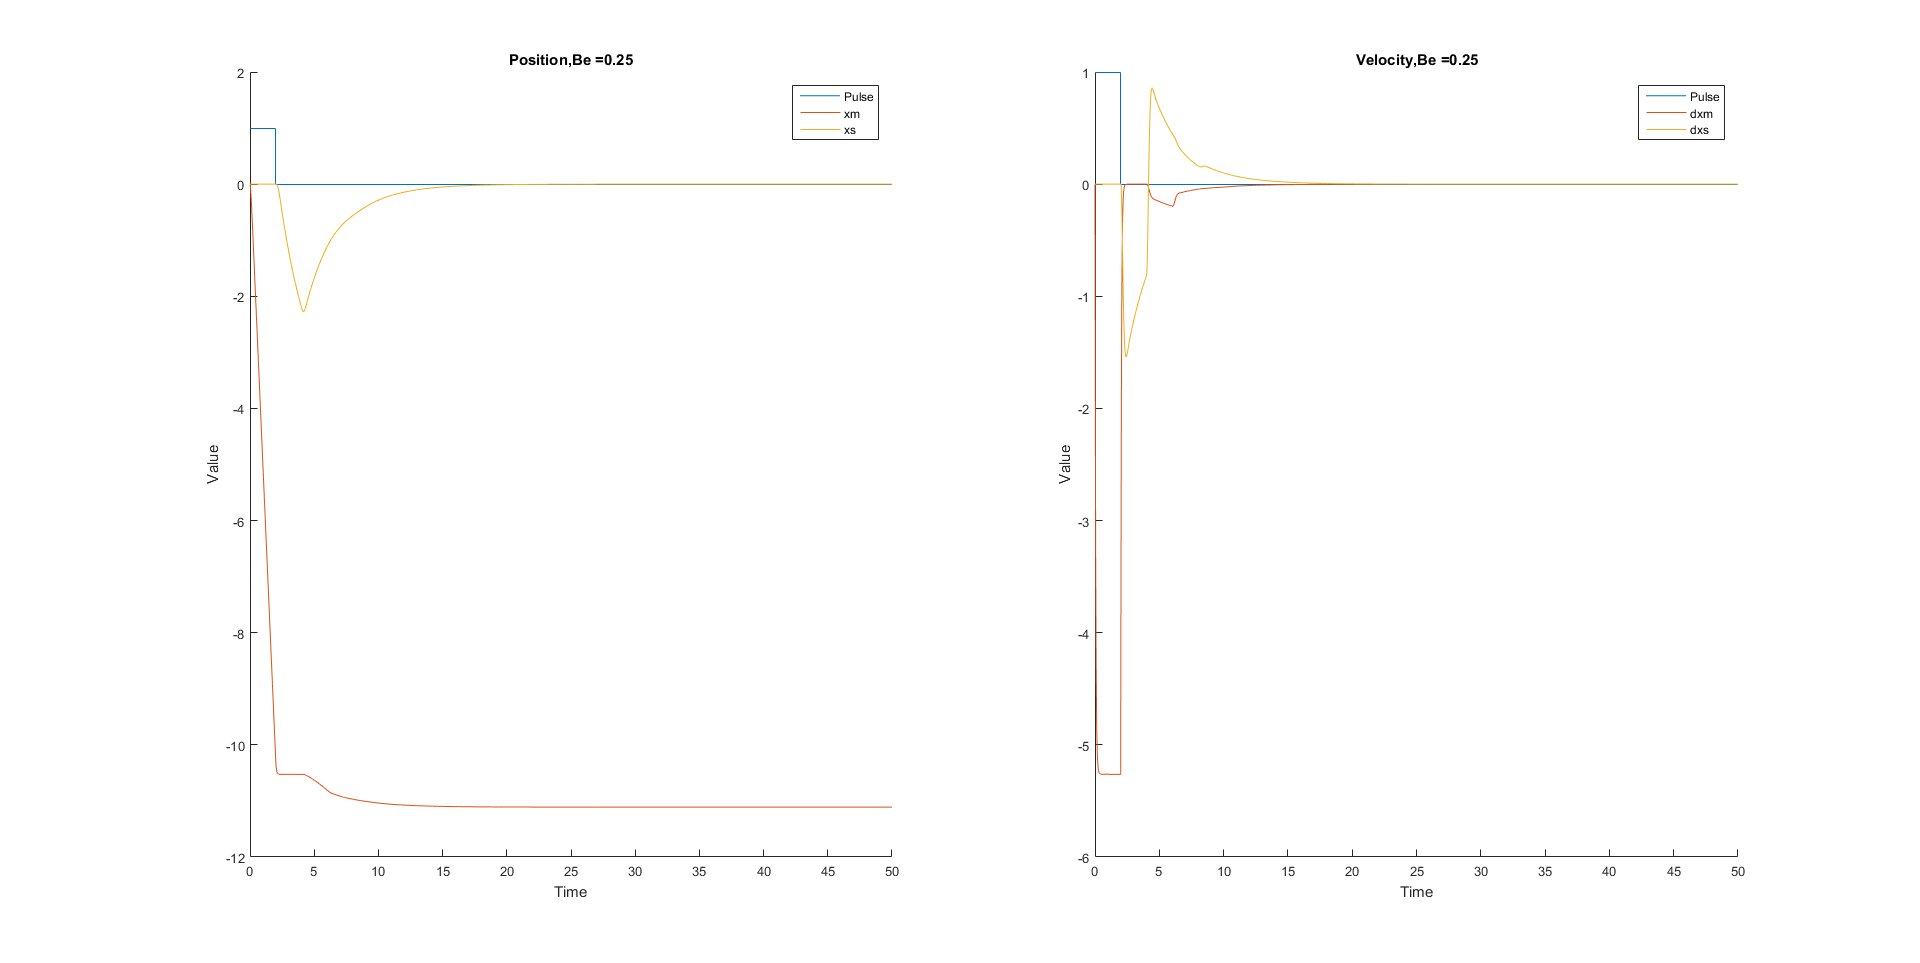
\includegraphics[width=1.0\linewidth]{images/Be025.png}
		\caption{Constante Fricción del Entorno, $B_e=0.25$}
		\label{BE025}
	\end{figure}
	
\end{frame}

\begin{frame}{Variando la Constante Fricción del Entorno}{$B_e=2.5$}
	
	\begin{figure}[h!]
		\centering
		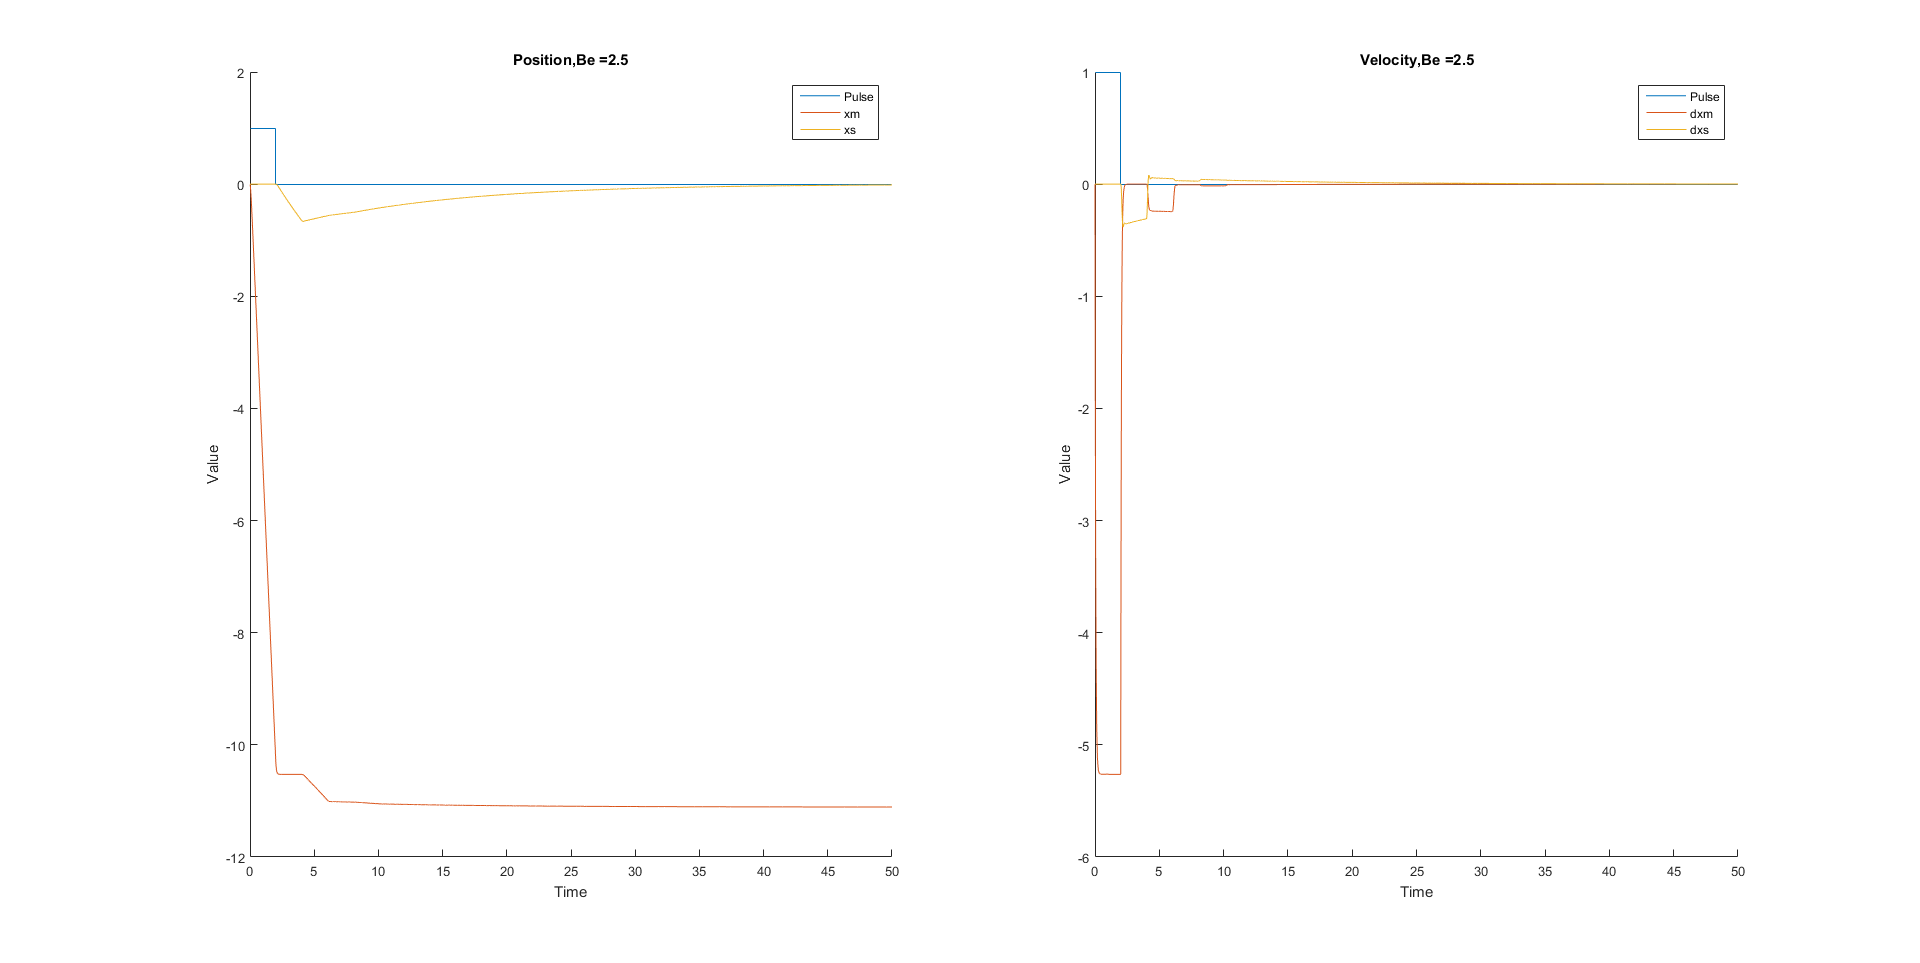
\includegraphics[width=1.0\linewidth]{images/Be25.png}
		\caption{Constante Fricción del Entorno, $B_e=2.5$}
		\label{BE25}
	\end{figure}
	
\end{frame}

\begin{frame}{Variando la Constante Fricción del Entorno}{$B_e=0$}
	
	\begin{figure}[h!]
		\centering
		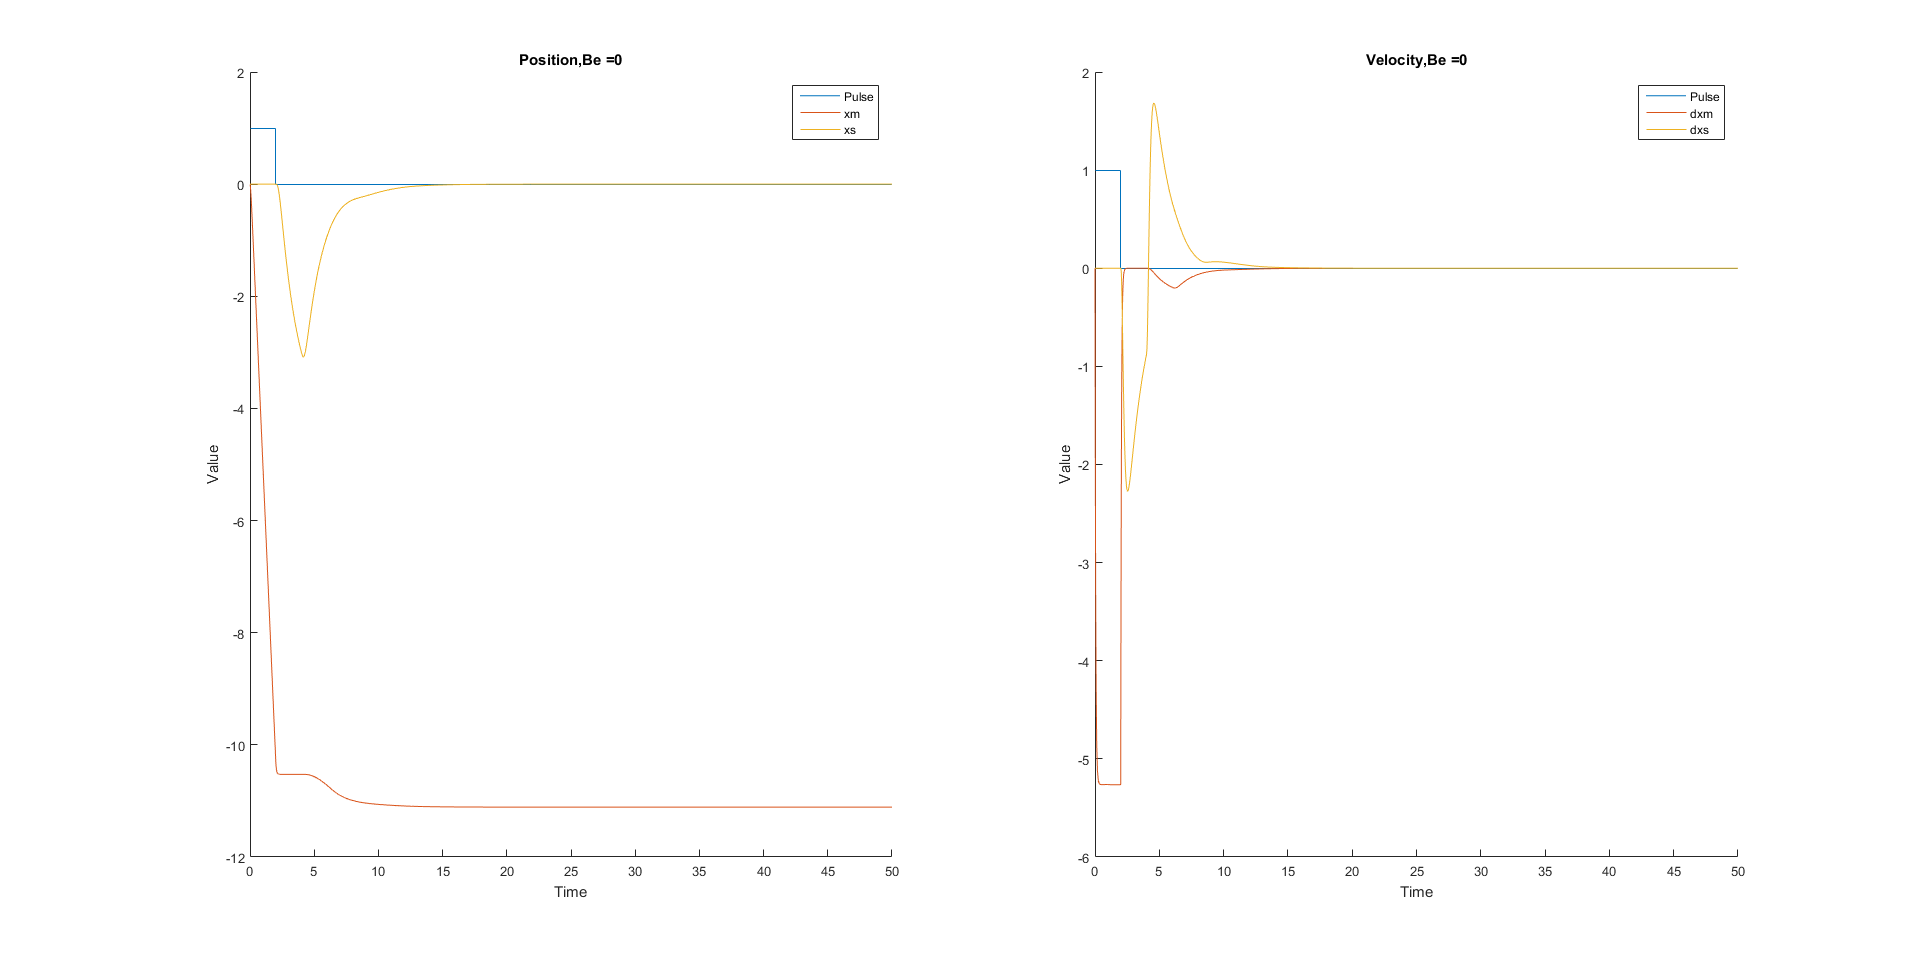
\includegraphics[width=1.0\linewidth]{images/Be0.png}
		\caption{Constante Fricción del Entorno, $B_e=0$}
		\label{BE0}
	\end{figure}
	
\end{frame}

\begin{frame}{Variando la Constante Elástica del Maestro}{$K_h=0.25$}
	
	\begin{figure}[h!]
		\centering
		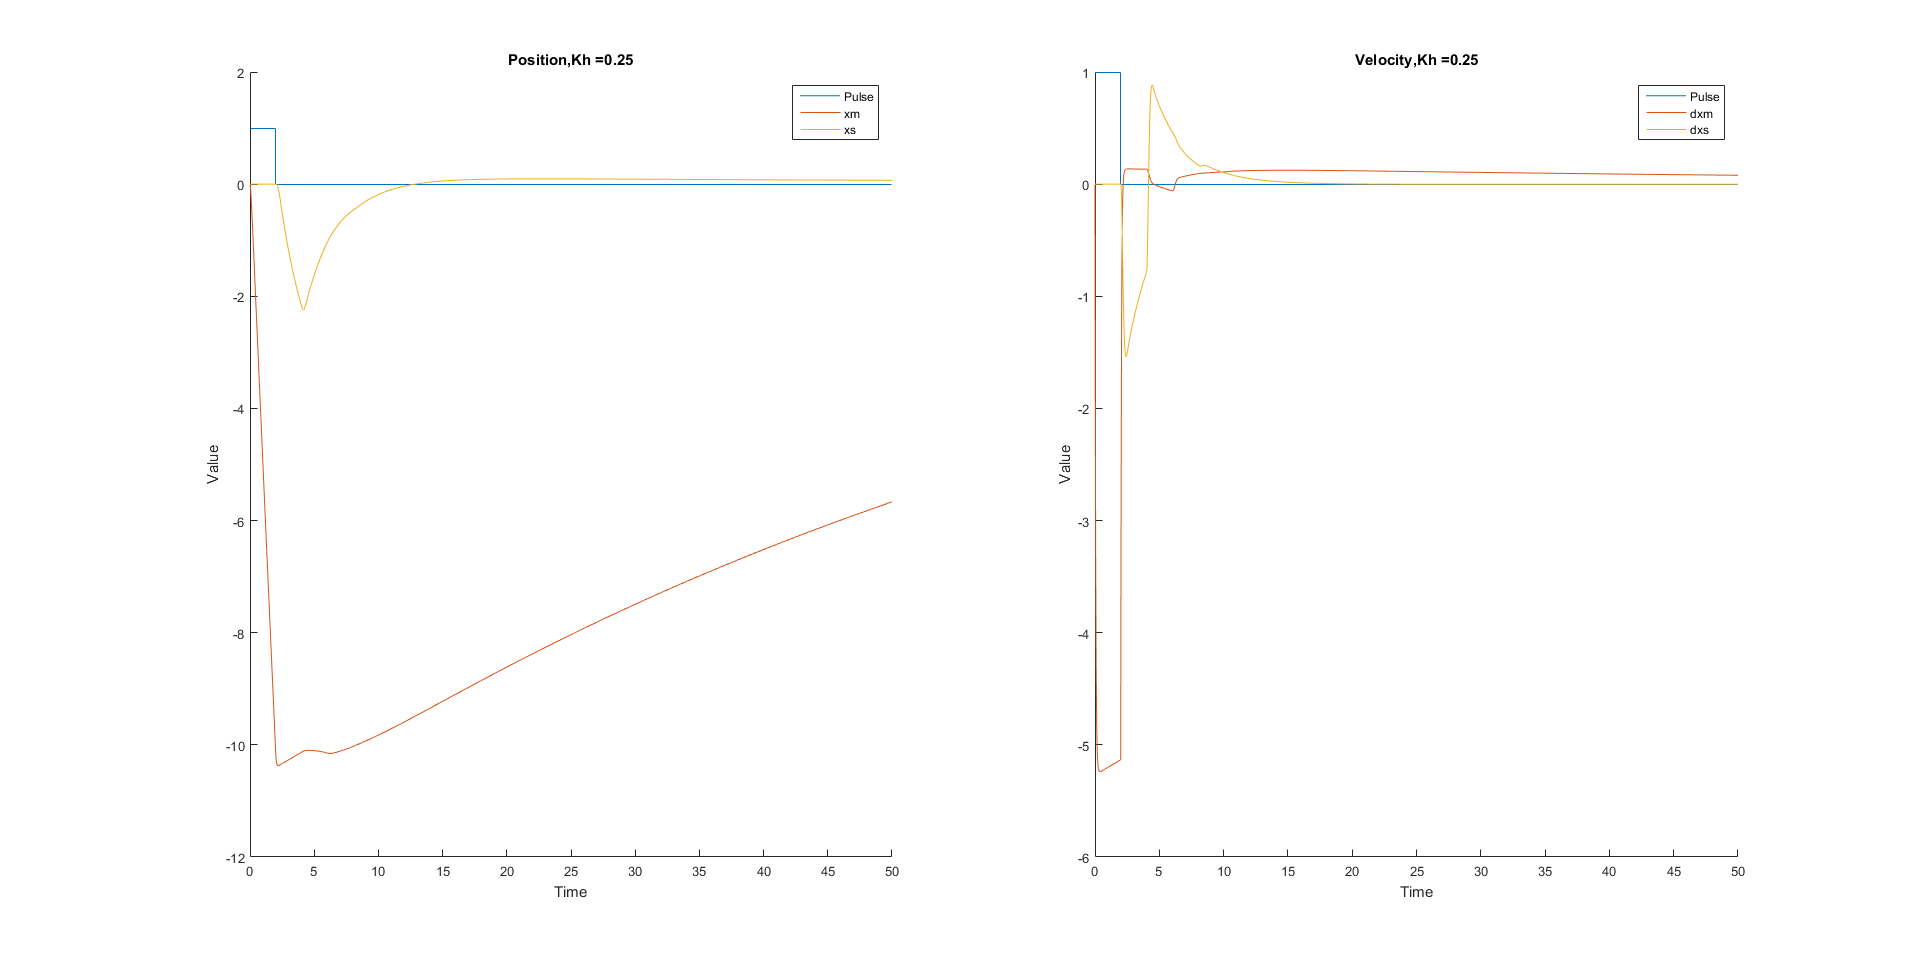
\includegraphics[width=1.0\linewidth]{images/Kh025.png}
		\caption{Constante Elástica del Maestro, $K_h=0.25$}
		\label{KH025}
	\end{figure}
	
\end{frame}

\begin{frame}{Variando la Constante Elástica del Maestro}{$K_h=1.25$}
	
	\begin{figure}[h!]
		\centering
		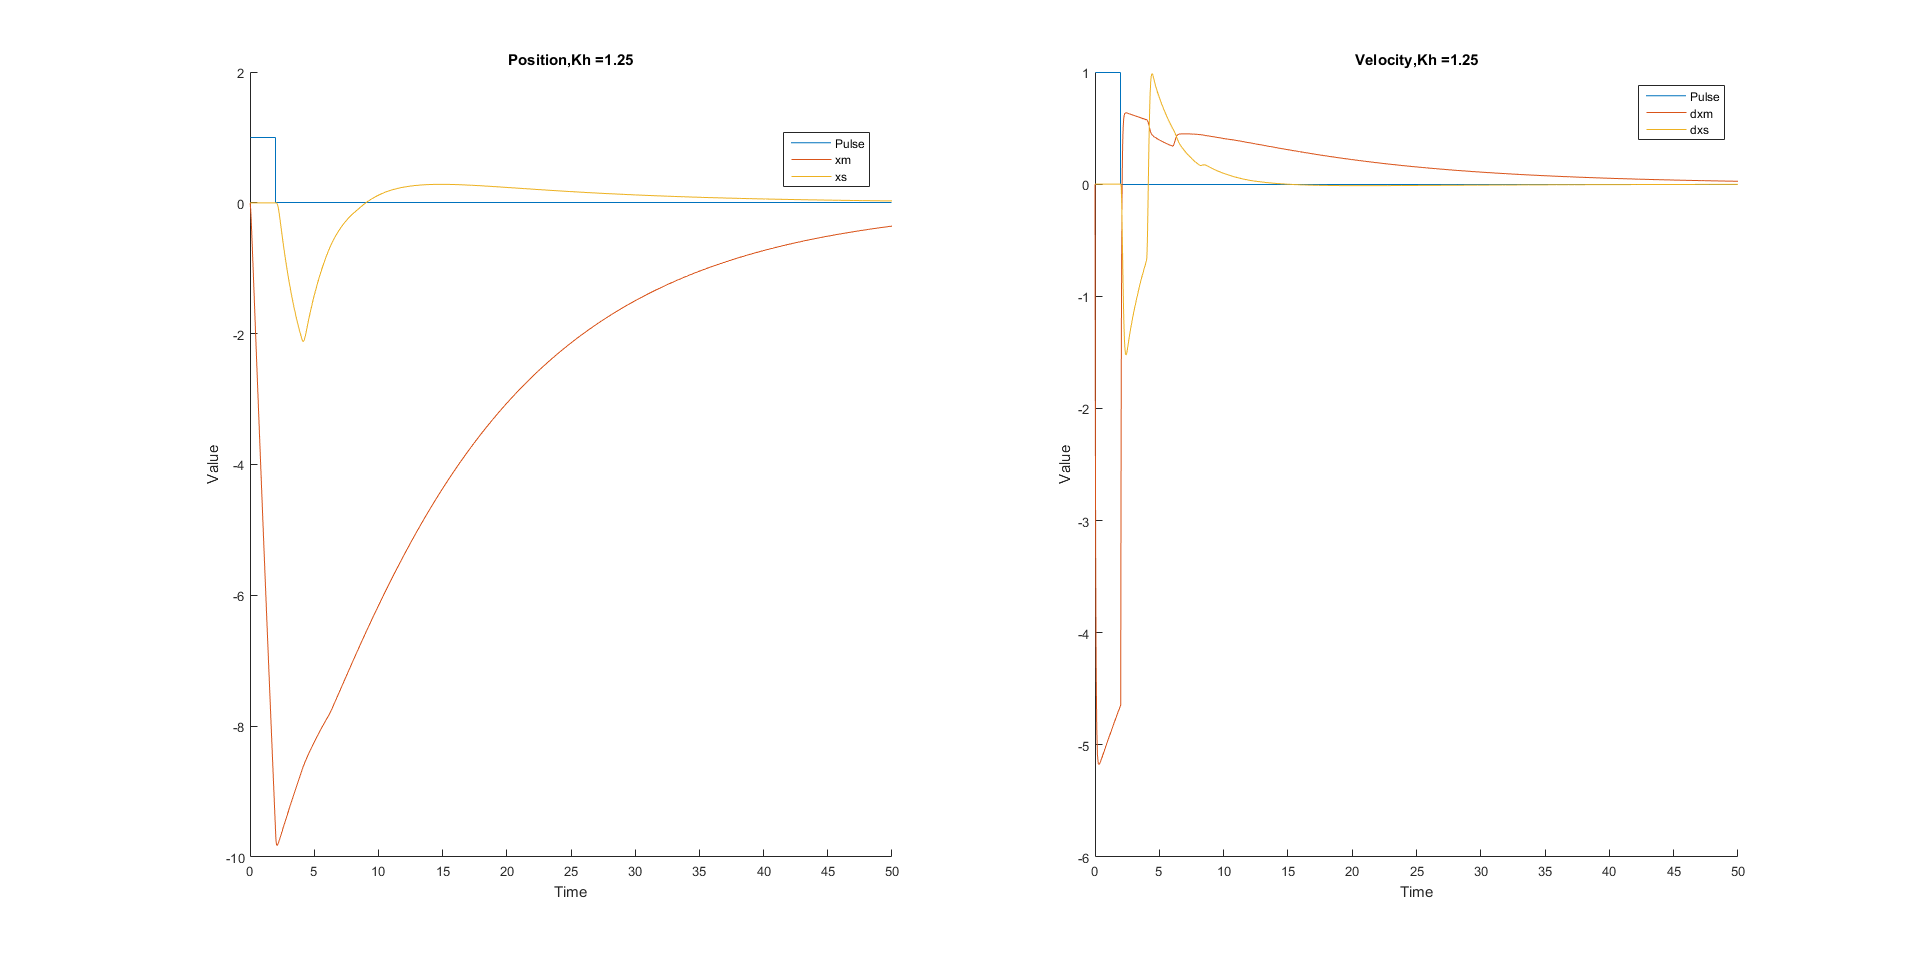
\includegraphics[width=1.0\linewidth]{images/Kh125.png}
		\caption{Constante Elástica del Maestro, $K_h=1.25$}
		\label{KH125}
	\end{figure}
	
\end{frame}

\begin{frame}{Variando la Constante Elástica del Maestro}{$K_h=2.5$}
	
	\begin{figure}[h!]
		\centering
		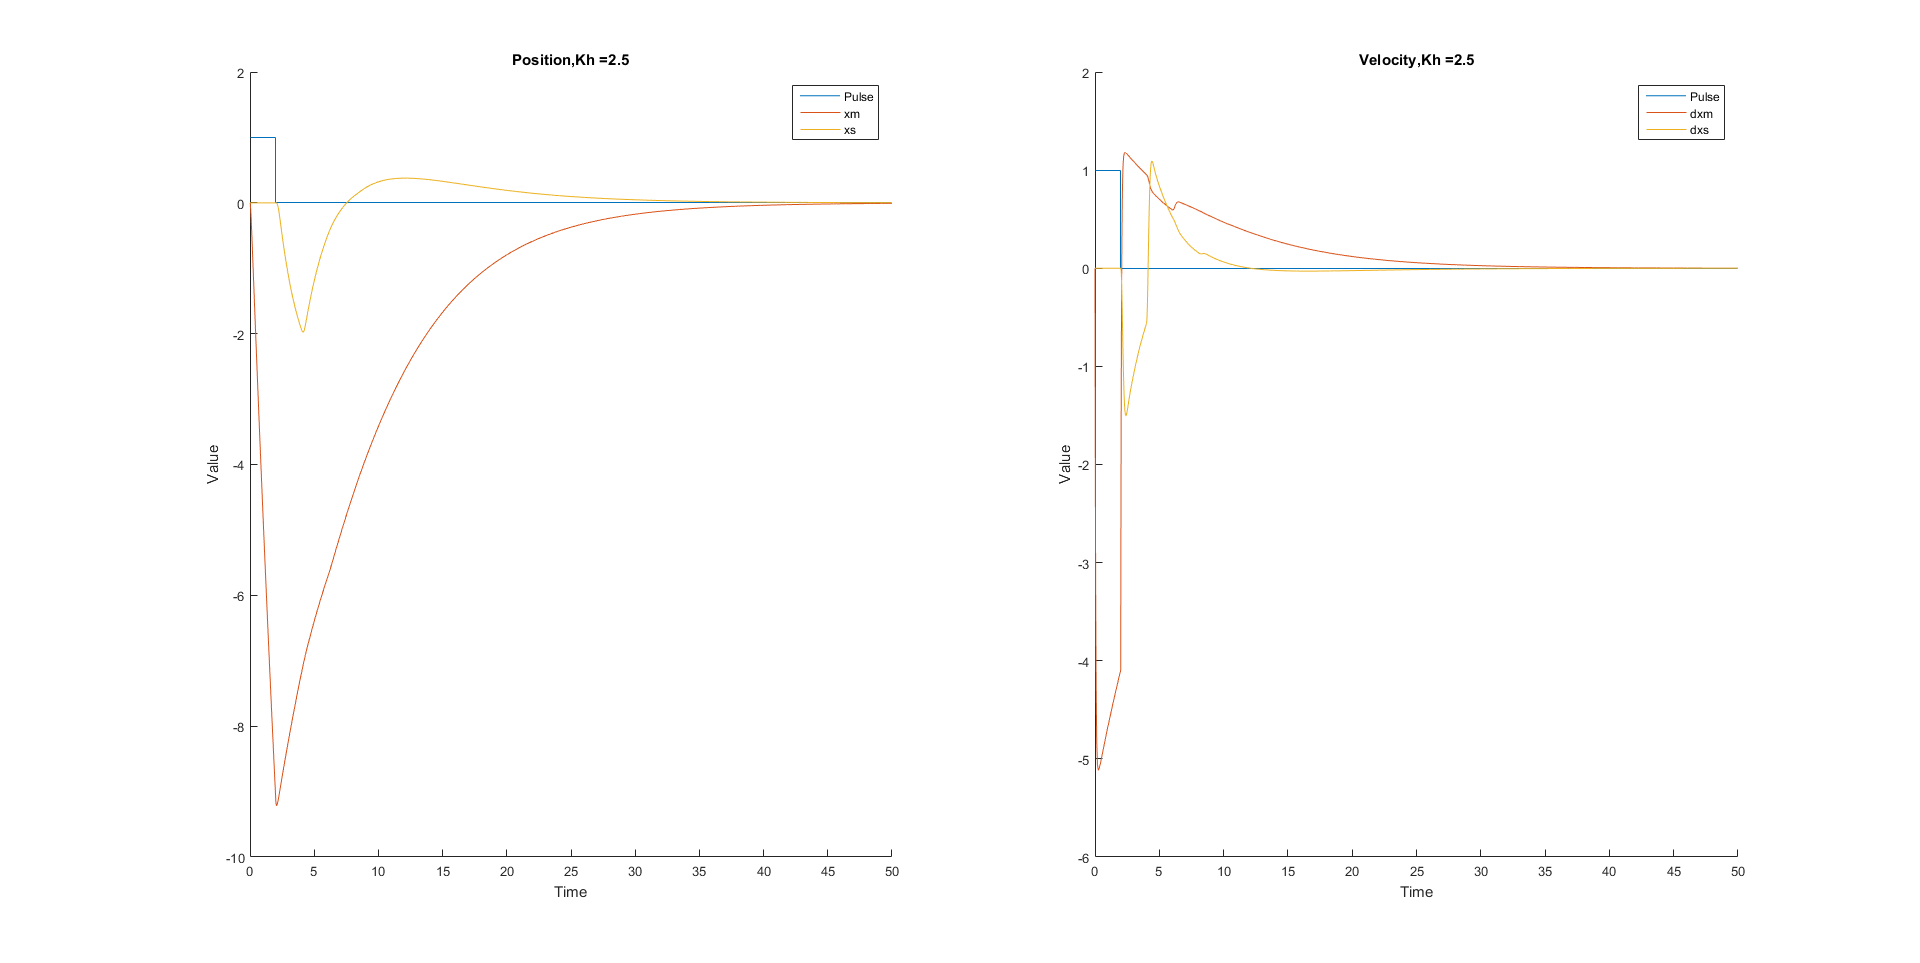
\includegraphics[width=1.0\linewidth]{images/Kh25.png}
		\caption{Constante Elástica del Maestro, $K_h=2.5$}
		\label{KH25}
	\end{figure}
	
\end{frame}

\begin{frame}
	\centering
	\LARGE{MUCHAS GRACIAS}\\
	\pause
	\bigskip
	\bigskip
	\Large{¿Preguntas?}
\end{frame}

% All of the following is optional and typically not needed. 
\appendix
\section<presentation>*{\appendixname}
\subsection<presentation>*{Bibliografía}

\begin{frame}[allowframebreaks]
  \frametitle<presentation>{Bibliografía}
    
  \begin{thebibliography}{10}
    
  \beamertemplatebookbibitems
  % Start with overview books.

  %\bibitem{Author1990}
  % A.~Author.
  % \newblock {\em Handbook of Everything}.
  % \newblock Some Press, 1990.
 
    
  \beamertemplatearticlebibitems
  % Followed by interesting articles. Keep the list short. 

  \bibitem{Chapter10}
  Sandra Hirche, Manuel Ferre, Jordi Barrio, Claudio Melchiorri, and Martin Buss
  \newblock Bilateral Control Architectures for Telerobotics
  \newblock {\em Advances in Telerobotics, chapter 10,
  	2007.}
  
  \bibitem{Chapter11}
  Manuel Ferre, Jordi Barrio, Claudio Melchiorri, Juan M. Bogado, Pedro L. Castedo, and Juan M. Ibarra
  \newblock Experimental Results on Bilateral Control Using
  an Industrial Telemanipulator
  \newblock {\em Advances in Telerobotics, chapter 11,
  	2007.}
  \end{thebibliography}
\end{frame}

\end{document}


